\documentclass[11pt,oneside]{report}
\usepackage{osnotes}

\begin{document}

\begin{titlepage}
  \raggedright
  \vspace*{2in}
  {\Huge\bfseries CSCI-GA 2250-002\par}
  \vspace{8pt}
  {\LARGE Operating Systems\par}
  \vspace{8pt}
  {\LARGE Course Notes\par}
  \vspace{8pt}
  {\Large Fall 2026\par}
  \vspace{24pt}
  {\large Instructor: Dr.\ Yang Tang\par}
  \vspace{4pt}
  {\large Notes by You Li\par}
\end{titlepage}

\thispagestyle{fancy}
\markright{}
{\Large\bfseries Acknowledgements\par}
\vspace{6pt}
These notes follow the Fall 2026 lectures of CSCI-GA 2250-002 (Operating Systems) at the Courant Institute, taught by Dr.\ Yang Tang. Each chapter follows one slide deck: \Cref{ch:intro} covers \emph{1 --- Introduction}, and \Cref{ch:proc} currently covers slides 2--162 of \emph{2 --- Process Management}. Sections marked (SUPPLEMENT) go beyond the slides and draw on Bryant and O'Hallaron~\cite{CSAPP}, Arpaci-Dusseau~\cite{OSTEP}, and Tanenbaum and Bos~\cite{MOS}.

\paragraph{Notation.} Code, commands, and file names are set in \code{typewriter}. A call such as \code{fork()} refers to the function; \code{man 2 fork} refers to section~2 of the manual (system calls), and section~3 holds library functions. Shell sessions begin with the prompt \code{\$}. PIDs in the examples (2436, 2437, \dots) follow the slides. Figures captioned ``after slide $n$'' redraw the corresponding slide; in timelines, a solid line means running, a dashed line means blocked or stopped, and a grey line marks a zombie.

\tableofcontents

\chapter{Introduction}
\label{ch:intro}

Supplementary reading:
\begin{itemize}
  \item \cite{MOS} Sections 1.1, 1.3, 1.5, and 1.6.
  \item \cite{OSC} Chapters 1 and 2.
  \item \cite{OSTEP} Chapter 2.
  \item \cite{CSAPP} Sections 1.7 and 8.1.
\end{itemize}

This chapter follows the slide deck \emph{1 --- Introduction}. It answers what an operating system is, shows the ways programs and people interact with it, and previews the abstractions the rest of the course is organized around:
\begin{itemize}
  \item \Cref{sec:what-os}: where the OS sits between users and hardware, and what happens when you type \code{ls};
  \item \Cref{sec:interact}: interrupts, system calls versus library calls, and kernel mode versus user mode;
  \item \Cref{sec:abstractions}: the four OS abstractions---processes, files, address spaces, and protection---that structure the course.
\end{itemize}

\section{What Is an Operating System?}
\label{sec:what-os}

\subsection{Where the OS Fits In}

Between a user and the computer hardware sits the operating system. Its job is to turn ugly hardware into beautiful abstractions. The OS hides the mechanics of the hard disk from you, for example, and lets you manipulate \emph{files} instead.

Users do not deal with the OS directly, though. They deal with \emph{processes}, the running images of programs. You have only one copy of Google Chrome, but you can open several browser windows from the same program file. Everything you run---accessing files, browsing the web, watching videos, playing games, doing the OS labs---runs as a process, which is why much of this course is about the process lifecycle, process management, and related issues.

\subsection{Example: What Happens When You Type \texorpdfstring{\code{ls}}{ls}}

When the user enters \code{ls}, which process runs, how does the OS react, and how does it work with the hardware to get the result back? \Cref{fig:ls} traces the five steps.

\begin{figure}[htbp]
\centering
\begin{tikzpicture}[col/.style={minimum height=34mm, anchor=south west, draw, font=\small, inner sep=0pt},
                    mod/.style={draw, fill=initc!30, font=\scriptsize, minimum width=17mm, minimum height=5mm}]
  \node[col, fill=tsk, minimum width=22mm] (u) at (0,0) {};
  \node[col, fill=uspace, minimum width=30mm] (p) at (u.south east) {};
  \node[col, fill=kspace, minimum width=30mm] (o) at (p.south east) {};
  \node[col, fill=childc!30, minimum width=30mm] (h) at (o.south east) {};
  \foreach \n/\t in {u/User, p/Processes, o/Operating System, h/Computer hardware}
    \node[anchor=south, font=\small] at ([yshift=1.5mm]\n.south) {\t};
  \node[pill, fill=orange!40, minimum width=11mm, minimum height=5mm, font=\scriptsize] at ([xshift=-7mm, yshift=8mm]p.center) {};
  \node[pill, fill=orange!40, minimum width=11mm, minimum height=5mm, font=\scriptsize\ttfamily] (ls) at ([xshift=6mm, yshift=1mm]p.center) {ls};
  \node[pill, fill=orange!40, minimum width=11mm, minimum height=5mm] at ([xshift=-5mm, yshift=-7mm]p.center) {};
  \node[mod] (mem) at ([yshift=9mm]o.center) {Memory};
  \node[mod] (fs) at ([yshift=-6mm]o.center) {File system};
  \node[draw, fill=white, font=\scriptsize, minimum width=14mm, minimum height=6mm] (disk) at ([yshift=-2mm]h.center) {Disk};
  \node[circle, draw, fill=orange!50, minimum size=6mm] (user) at ([yshift=3mm]u.center) {};
  \draw[fill=kernc!50] ([yshift=-1mm]user.south) ++(-5mm,-4mm) arc (180:0:5mm) -- cycle;
  \draw[arr, sigc] (user) -- node[above, font=\scriptsize]{(1)} (ls);
  \draw[arr, sigc] (ls) -- node[below left=-1mm, font=\scriptsize]{(2)} (fs);
  \draw[arr, sigc] (fs) -- node[below, font=\scriptsize]{(3)} (disk);
  \draw[arr, sigc] (disk) -- node[above, font=\scriptsize]{(4)} (mem);
  \draw[arr, sigc] (mem) -- node[above, font=\scriptsize]{(5)} (ls);
  \draw[{Stealth[length=1.6mm]}-{Stealth[length=1.6mm]}, thick, accent] ([yshift=4mm]u.north east) ++(-6mm,0) -- ++(12mm,0)
    node[above, font=\scriptsize, align=center, pos=0.5, yshift=1mm, color=black] {keyboard, mouse,\\voice, \dots};
  \draw[{Stealth[length=1.6mm]}-{Stealth[length=1.6mm]}, thick, accent] ([yshift=4mm]p.north east) ++(-6mm,0) -- ++(12mm,0)
    node[above, font=\scriptsize, align=center, pos=0.5, yshift=1mm, color=black] {programming interface\\(system calls)};
  \draw[{Stealth[length=1.6mm]}-{Stealth[length=1.6mm]}, thick, accent] ([yshift=4mm]o.north east) ++(-6mm,0) -- ++(12mm,0)
    node[above, font=\scriptsize, align=center, pos=0.5, yshift=1mm, color=black] {machine\\language};
\end{tikzpicture}
\caption{The OS between processes and hardware, and the five steps of running \code{ls}; the arrows on top are the three interfaces between neighboring layers (after slides 9--15).}
\label{fig:ls}
\end{figure}

\begin{enumerate}
  \item Most commands typed in the shell start a new process, here one running \code{ls}.
  \item \code{ls} asks the OS to read the directory. The OS contains the code needed to work with the file system; such code in the OS is called the \emph{kernel}.
  \item The file system module knows how to work with devices through \emph{device drivers}, and issues I/O requests to the disk.
  \item The OS allocates memory for the results.
  \item The memory management subsystem copies the results into the memory of the \code{ls} process, which prints them.
\end{enumerate}

\begin{definition}[Kernel]
  The \emph{kernel} is the core of the operating system: the code, together with its data, that manages the hardware and provides services such as file systems, memory management, and process management to processes.
\end{definition}

\subsection{Two Viewpoints}

\begin{definition}[Operating System]
  An \emph{operating system} is a piece of software seen from two viewpoints.
  \begin{itemize}
    \item \emph{Top-down}: the OS is an \emph{extended machine}. It provides a clean abstraction through which processes access the machine.
    \item \emph{Bottom-up}: the OS is a \emph{resource manager}. It manages all parts of the system efficiently.
  \end{itemize}
\end{definition}

The rest of the course discusses the details of OS design from both angles.

\subsection{(SUPPLEMENT) Further Topics}
\label{sec:what-os-further}

\paragraph{The kernel is not the whole OS.} What ships as ``the operating system'' includes the kernel plus user-space programs: the shell, system libraries such as \code{libc}, \code{init}/systemd, utilities like \code{ls}. Only the kernel runs in kernel mode (\Cref{sec:interact}). The shell, in particular, is an ordinary program (\Cref{sec:abstractions}).

\paragraph{Monolithic kernels and microkernels.} Linux is a \emph{monolithic} kernel: file systems, drivers, memory and process management all run in kernel mode in one address space, which is fast but means a driver bug can crash the whole system. Loadable modules (\code{lsmod}, \code{modprobe}) add code at run time without changing this. A \emph{microkernel} (Mach, seL4, QNX) keeps only scheduling, memory mapping, and message passing in the kernel and runs file systems and drivers as user-space servers, trading speed for isolation. macOS's XNU and Windows NT are hybrids.

\paragraph{Watching the steps happen.} \code{strace ls} prints every system call \code{ls} makes: \code{openat} on the directory, \code{getdents64} to read its entries, \code{write} to print them. It is the user-visible trace of steps (2)--(5) above.

\section{Interacting with the OS}
\label{sec:interact}

\subsection{Three Points of View}

Who interacts with the OS, and how, depends on who you are.
\begin{itemize}
  \item \emph{An ordinary user} sees the OS as something that runs programs, through the keyboard, the mouse, voice recognition, and so on. They need not even know what a process is---unless Google Chrome freezes and must be killed.
  \item \emph{A software engineer} sees the OS as software that lets a program interact with the user, the hardware, or the OS itself, through \emph{system calls}.
  \item \emph{A hardware engineer} sees the OS as software that hosts \emph{device drivers}. How does the computer handle input and output? What happens when the user types a key?
\end{itemize}

\subsection{Interrupts}

Answering the last question requires a little computer architecture. The CPU is executing some program code, and its \emph{program counter} register points to the next instruction to be executed. Suddenly someone types a key.

\begin{definition}[Interrupt]
  A \emph{hardware interrupt} is a signal from a device asking the CPU to interrupt the currently executing code (when permitted) so that the device's event can be processed in a timely manner. Each kind of interrupt has a unique \emph{interrupt number}, and the \emph{interrupt vector} is an array of addresses, indexed by interrupt number, pointing to the \emph{interrupt handlers}.
\end{definition}

\begin{figure}[htbp]
\centering
\begin{tikzpicture}
  \node[draw, fill=white, font=\scriptsize, minimum width=16mm, minimum height=7mm] (kb) at (-3.4,0) {Keyboard};
  \node[field, minimum width=24mm] (pc) at (0,0) {Program counter};
  \node[font=\small\bfseries, above=1mm of pc] (cpu) {CPU};
  \begin{scope}[on background layer]
    \node[fit=(pc)(cpu), fill=initc!25, draw=initc!70, rounded corners=3pt] (CPU) {};
  \end{scope}
  \draw[arr, childc, line width=1.4pt] (kb) -- node[above, font=\scriptsize, color=black]{interrupt} (CPU);
  \node[draw, fill=uspace, font=\scriptsize, minimum width=12mm] (code) at (3.4,-1.7) {Code};
  \node[font=\scriptsize] (ivt) at (6.0,2.3) {Interrupt vector};
  \fieldstack[field, minimum width=13mm, minimum height=5mm]{v}{ivt.south}{0, 1, 2, \dots, 255}
  \node[draw, fill=kspace, font=\scriptsize, align=center] (dz) at (9.0,1.85) {Divide-by-zero\\interrupt handler};
  \node[draw, fill=kspace, font=\scriptsize, align=center] (kh) at (9.0,-0.6) {Keyboard\\interrupt handler};
  \draw[arr, densely dashed] (v-1.east) -- (dz.west |- v-1);
  \draw[arr, densely dashed] (v-4.east) -- (kh.west);
  \draw[arr] (pc.east) -- node[below, sloped, font=\scriptsize]{(1) transfer control} (kh.south west);
  \draw[arr, kernc] (kh.south) to[out=-110, in=0] node[below, font=\scriptsize, pos=0.5]{(2) return} (code.east);
  \draw[densely dotted] (pc.south) |- (code.west);
\end{tikzpicture}
\caption{Handling a keyboard interrupt (after slides 19--23). The CPU looks up the handler in the interrupt vector, transfers control to it, and the handler returns to the interrupted code.}
\label{fig:interrupt}
\end{figure}

As \Cref{fig:interrupt} shows, the CPU transfers control to the handler for that interrupt number, the handler processes the interrupt, and finally it returns control to the original code. Seen from the hardware side, then, the programs on a computer are just processes running on top of the OS, and they interact with it through system calls.

\subsection{System Calls}

\begin{definition}[System Call]
  A \emph{system call} (syscall) looks like an ordinary function call, with one important distinction: its implementation is inside the OS kernel. Invoking a system call \emph{traps} into the kernel. System calls are the programming interface between processes and the kernel.
\end{definition}

\begin{example}[\code{time()}]
\begin{lstlisting}
int add(int a, int b) {
  return a + b;
}
int main() {
  int s = add(1, 2);        // ordinary function call
  time_t t = time(NULL);    // system call: traps into the kernel
}
\end{lstlisting}
  A process is running \code{main}. When it calls \code{time()}, it asks the kernel to run the \code{time()} system call; the kernel asks the hardware clock for the current time and returns the result. Note that the kernel is \emph{not} an executing entity of its own: it is a body of compiled code and allocated memory, run by the process that trapped into it.
\end{example}

System calls are usually primitive and fundamental; \code{time()} just tells you what time it is. An OS provides system calls for process control, file management, device management, information maintenance, communications, and protection. \emph{POSIX} (the Portable Operating System Interface) standardizes a common set. To check whether a function is a system call, consult \code{man syscalls}, the list of Linux system calls (section 2 of the manual).

\subsection{System Calls vs.\ Library Calls}

Which of \code{abs()}, \code{fopen()}, \code{fread()}, \code{malloc()}, \code{memcpy()}, and \code{printf()} are system calls? None of them.

\begin{definition}[Library Function]
  A \emph{library function} is an ordinary function implemented in a library, not in the kernel. Library functions are compiled and packed into library files: \code{*.so} (shared object) on Linux, \code{*.dylib} (dynamic library) on macOS, and \code{*.dll} (dynamic-link library) on Windows.
\end{definition}

A library function may itself invoke system calls. \code{fopen()}, implemented in the standard C library (e.g., \code{/lib/libc-2.17.so}), invokes the system call \code{open()}. Why reinvent the wheel? Because system calls are often too primitive and not programmer-friendly. Compare
\begin{lstlisting}
open("file.txt", O_CREAT|O_WRONLY|O_TRUNC, S_IRUSR|S_IWUSR);
fopen("file.txt", "w");
\end{lstlisting}

\subsection{Kernel Mode and User Mode}

\begin{definition}[Kernel Mode and User Mode]
  The CPU has (at least) two separate modes of operation. The OS runs in \emph{kernel mode} (a.k.a.\ privileged mode), with complete access to all the hardware and the ability to execute any instruction. All other programs run in \emph{user mode}: only a subset of the machine instructions is available, and they cannot affect control of the machine or do I/O.
\end{definition}

\begin{figure}[htbp]
\centering
\begin{tikzpicture}[mod/.style={draw, font=\scriptsize, align=center, minimum width=19mm, minimum height=9mm}]
  \fill[uspace] (-1.4,1.3) rectangle (12.6,3.1);
  \fill[kspace] (-1.4,-2.7) rectangle (12.6,1.2);
  \draw[dashed, cmt] (-1.4,1.25) -- (12.6,1.25);
  \node[anchor=west, font=\small\bfseries, color=parentc!70!black] at (-1.3,2.8) {User mode};
  \node[anchor=west, font=\small\bfseries, color=kernc] at (-1.3,0.9) {Kernel mode};
  \node[draw, fill=white, font=\scriptsize, minimum width=18mm, minimum height=8mm] (app) at (1.6,2.1) {Application};
  \node[draw, fill=termbg, font=\scriptsize\ttfamily, minimum width=26mm, minimum height=8mm] (libc) at (8.0,2.1) {/lib/libc-2.17.so};
  \node[draw, fill=tsk, font=\small, minimum width=110mm, minimum height=7mm] (sc) at (5.4,0.25) {System calls};
  \node[mod, fill=childc!35] (dd) at (2.0,-1.3) {Device\\drivers};
  \node[mod, fill=kspace!60!kernc!40] (fs) at (4.6,-1.3) {File\\systems};
  \node[mod, fill=jobC!70] (mm) at (7.2,-1.3) {Memory\\management};
  \node[mod, fill=parentc!35] (pm) at (9.8,-1.3) {Process\\management};
  \node[font=\small] at (11.7,-1.3) {\dots};
  \node[draw, fill=greybg, font=\scriptsize, minimum width=12mm, minimum height=7mm] (disk) at (-0.4,-2.1) {Disk};
  \tikzset{down/.style={arr, sigc}, up/.style={arr, kernc}, n/.style={font=\scriptsize, fill=white, inner sep=1pt}}
  \draw[down] ([yshift=1.2mm]app.east) -- node[n, pos=0.3]{1} ([yshift=1.2mm]libc.west);
  \draw[up] ([yshift=-1.2mm]libc.west) -- node[n, pos=0.3]{11} ([yshift=-1.2mm]app.east);
  \draw[down] ([xshift=-2mm]libc.south) -- node[n]{3} ([xshift=-2mm]libc.south |- sc.north);
  \draw[up] ([xshift=2mm]libc.south |- sc.north) -- node[n]{10} ([xshift=2mm]libc.south);
  \draw[down] ([xshift=-2mm]fs.north |- sc.south) -- node[n]{4} ([xshift=-2mm]fs.north);
  \draw[up] ([xshift=2mm]fs.north) -- node[n]{9} ([xshift=2mm]fs.north |- sc.south);
  \draw[down] ([yshift=1.2mm]fs.west) -- node[n]{5} ([yshift=1.2mm]dd.east);
  \draw[up] ([yshift=-1.2mm]dd.east) -- node[n]{8} ([yshift=-1.2mm]fs.west);
  \draw[down] ([yshift=-1.5mm]dd.south west) -- node[n]{6} ([yshift=1.5mm]disk.east);
  \draw[up] ([yshift=-1.5mm]disk.east) -- node[n]{7} ([yshift=-3.5mm]dd.south west);
  \node[font=\scriptsize, anchor=west] at ([xshift=1mm]libc.east) {2: library wrapper};
\end{tikzpicture}
\caption{Opening a file with \code{fopen()} (after slides 35--36). Red: the request travels down; blue: the result travels back up.}
\label{fig:fopen}
\end{figure}

\begin{example}[\code{fopen()} Across the Mode Boundary]
  \Cref{fig:fopen} numbers the steps.
  \begin{enumerate}
    \item The application calls \code{fopen()} in user mode.
    \item The C library's wrapper prepares the request.
    \item It calls \code{open()}, which TRAPs into the OS kernel.
    \item The kernel allocates kernel data structures and hands the request to the file system.
    \item The file system asks the device driver to read the file's metadata.
    \item The driver issues a low-level disk read command.
    \item The data is stored in memory.
    \item The driver returns the file's metadata to the file system.
    \item The file system finishes the open.
    \item The system call returns the low-level \emph{file descriptor} with RETURN-FROM-TRAP, back in user mode.
    \item The library returns the high-level \emph{file pointer} (\code{FILE *}) to the application.
  \end{enumerate}
\end{example}

\Cref{sec:kernel} looks inside steps 3 and 10: how the kernel finds the right handler for a system call, and what a file descriptor is.

\subsection{(SUPPLEMENT) Further Topics}
\label{sec:interact-further}

\paragraph{Interrupts, traps, and faults.} The slides use ``interrupt'' broadly. A common taxonomy distinguishes \emph{interrupts}, asynchronous events from devices such as the keyboard or the timer; \emph{traps}, synchronous and intentional, such as a system call; and \emph{faults} (exceptions), synchronous and unintentional, such as division by zero or a page fault. All three enter the kernel through the same table. On x86 it is the 256-entry interrupt descriptor table, whose vector $0$ is indeed the divide error; device interrupts are remapped above the first $32$ vectors reserved for exceptions.

\paragraph{The answer to the quiz.} \code{abs()} and \code{memcpy()} make no system call at all. \code{printf()} and \code{fread()} buffer data and call \code{write()} and \code{read()} only when needed; \code{fopen()} calls \code{open()} (\code{openat()} in modern glibc); \code{malloc()} manages the heap itself and calls \code{brk()} or \code{mmap()} only to grow it. \code{man 2} pages are system calls and \code{man 3} pages are library functions.

\paragraph{Seeing system calls.} \code{strace ./prog} lists every system call a program makes, with arguments and return values; \code{ltrace} does the same for library calls. On modern systems the C library is \code{libc.so.6} (glibc 2.34 and later); \code{/lib/libc-2.17.so} on the slides is from CentOS 7.

\paragraph{Why the mode bit is hardware.} If user mode were enforced by software, a program could simply skip the check. Because the CPU itself refuses privileged instructions in user mode and raises an exception instead, the OS can let untrusted programs run directly on the processor at full speed and still keep control. The only way back to kernel mode is through the entry points the kernel installed (the trap and interrupt tables), which is what makes the system call interface a security boundary.

\paragraph{The timer interrupt.} Interrupts are also how the OS regains the CPU from a program that never makes a system call: a hardware timer interrupts periodically and the kernel's handler can switch to another process. Preemptive scheduling (\Cref{sec:sched}) depends on it.

\section{OS Abstractions and Course Structure}
\label{sec:abstractions}

The OS provides four abstractions, and the course is organized around them:
\begin{center}
\begin{tabular}{ll}
  \toprule
  Abstraction & Parts of the course \\
  \midrule
  processes & Part 2: process management; Part 3: process synchronization \\
  address spaces & Part 4: memory management \\
  files & Part 5: storage management; Part 6: file system \\
  security and protection & Part 7: security and protection \\
  \bottomrule
\end{tabular}
\end{center}

\subsection{Processes}

Consider the two commands \code{ls} and \code{ls /}. Both use the same program file, \code{/bin/ls}. They differ in their program arguments and in the internal state of their processes, such as running time.

\begin{definition}[Process]
  A \emph{process} is an execution instance of a program. Multiple processes can execute the same program code, and a process is not bound to execute just one program. A process is an \emph{active} entity: it maintains local state about its execution---which CPU core it runs on, which instruction is next, \dots---and that state changes over time.
\end{definition}

\Cref{sec:program} returns to the distinction between program and process from the build side.

\begin{definition}[Shell]
  The \emph{shell}, the Unix command interpreter, is not part of the OS but an important program shipped with it. A shell starts when you log in, and it creates processes: when you enter a command, the shell, as the \emph{parent} process, creates a \emph{child} process that executes the command.
\end{definition}

The shell itself has a parent, and children may have children of their own, so all processes form a \emph{process tree} (\Cref{sec:org}). On a CIMS compute server:
\begin{lstlisting}[style=sh]
$ pstree
systemd-+-sshd---bash---pstree
        ...
\end{lstlisting}
systemd is the ancestor of all processes, \code{sshd} is the SSH server, and \code{bash} is the shell. Inside a Docker container the tree looks different, since the container is a virtualized environment. The \code{ps} command displays information about processes, including each one's \emph{PID} (process ID), a unique identification number:
\begin{lstlisting}[style=sh]
$ ps
  PID TTY          TIME CMD
 2250 pts/23   00:00:00 bash
 2436 pts/23   00:00:00 ps
$ ps aux
USER   PID %CPU %MEM    VSZ  RSS TTY  STAT START    TIME COMMAND
root     1  0.0  0.0 194812 8008 ?    Ss   Jan14  121:09 /usr/lib/systemd/systemd
root     2  0.0  0.0      0    0 ?    S    Jan14    0:27 [kthreadd]
...
\end{lstlisting}

On processes, the course covers process-related functions and system calls (how to write a shell yourself, Lab~2), the process lifecycle and scheduling (how processes are created and how their death is handled), process control (how to suspend a process, what Ctrl-C does and how to change it), and process synchronization and deadlocks (how processes communicate and cooperate, Lab~3). \Cref{ch:proc} begins this part.

\subsection{Files}

\begin{definition}[File and File System]
  A \emph{file} is a logical unit of information created by a process; think of it as an array of bytes, each of which you can read or write. A \emph{file system} (FS) is how the OS uses a storage device to manage files: it maintains files, directories, allocated space, and free space.
\end{definition}

Examples include APFS, ext4, FAT32, and NTFS. A file system is independent of the OS, and one OS can support several. File systems can be studied from two viewpoints: the \emph{static} view asks how files are stored on the disk, and the \emph{dynamic} view asks how the operations that update files are supported.

\begin{example}[Fundamental File Operations]
  Of \code{create}, \code{open}, \code{read}, \code{write}, \code{close}, \code{copy}, \code{delete}, \code{rename}, and \code{move}, not all are fundamental. \code{create} is a special case of \code{open}; \code{copy} can be implemented with \code{open}, \code{read}, and \code{write}; and \code{move} within the same file system is just \code{rename}.
\end{example}

On files, the course covers file-related functions and system calls, file system implementation (how well-known file systems work, why a file system becomes slow, how to recover a deleted file and why that does not always work, Lab~4, why a file can be lost on a physically healthy disk), and disks (what is inside a hard disk drive, and how multiple disks combine for performance, reliability, or both).

\subsection{Address Spaces}

When you run a program, it is loaded from the hard disk into main memory, and during execution its instructions are fetched from main memory into the CPU (\Cref{fig:hierarchy}). There may be a hundred processes running ``at the same time'' with only a few CPU cores; \Cref{sec:sched} explains how.

\begin{figure}[htbp]
\centering
\begin{tikzpicture}[pp/.style={draw, rounded corners=2.5mm, fill=orange!40, font=\scriptsize, minimum height=5mm, align=center}]
  \node[draw, fill=uspace, rounded corners=2pt, minimum width=36mm, minimum height=22mm, label={[font=\small\bfseries]above:CPU}] (cpu) at (0,0) {};
  \node[draw, fill=initc!30, font=\scriptsize, minimum width=12mm] at ([xshift=-10mm, yshift=4mm]cpu.center) {Registers};
  \node[draw, fill=initc!30, font=\scriptsize, minimum width=12mm] at ([xshift=10mm, yshift=4mm]cpu.center) {Cache};
  \node[pp] at ([yshift=-5mm]cpu.center) {Process A (running)};
  \node[draw, fill=kspace, rounded corners=2pt, minimum width=36mm, minimum height=22mm, label={[font=\small\bfseries]above:Main memory}] (mm) at (5.2,0) {};
  \node[pp] at ([xshift=-9mm, yshift=5mm]mm.center) {Process B};
  \node[pp] at ([xshift=9mm, yshift=0mm]mm.center) {Process C};
  \node[pp] at ([xshift=-7mm, yshift=-6mm]mm.center) {Process D};
  \node[draw, fill=kernc!30, rounded corners=6pt, minimum width=32mm, minimum height=22mm, label={[font=\small\bfseries]above:Disk}] (dk) at (10.2,0) {};
  \node[pp] at ([xshift=-6mm, yshift=4mm]dk.center) {Process E};
  \node[pp] at ([xshift=6mm, yshift=-5mm]dk.center) {Process F};
  \draw[arr] (mm) -- (cpu);
  \draw[arr] (dk) -- (mm);
\end{tikzpicture}
\caption{The memory hierarchy: programs move from disk to main memory to the CPU, and only a few processes run at any instant (after slide 52).}
\label{fig:hierarchy}
\end{figure}

\begin{definition}[Address Space]
  The \emph{address space} of a process is the range of (virtual) memory addresses it can use. A loader lays out the program in it as \emph{segments}: text (program code), initialized data, uninitialized data, the heap, mapped files, and the stack. This organization is called \emph{segmentation}.
\end{definition}

\begin{figure}[htbp]
\centering
\begin{tikzpicture}
  \node[font=\scriptsize\bfseries] (ct) at (0,0.1) {C program layout};
  \fieldstack[seg, fill=kspace, minimum width=36mm, minimum height=7mm]{c}{ct.south}{Program code, Constants, Global variables, Dynamically allocated memory, Local variables}
  \node[draw, ellipse, fill=tsk!80, minimum width=18mm, minimum height=36mm, font=\small] (ld) at (4.1,-1.9) {Loader};
  \node[font=\scriptsize\bfseries] (at) at (8.2,0.1) {Virtual address space};
  \fieldstack[seg, fill=uspace, minimum width=27mm]{a}{at.south}{Text, Initialized data, Uninitialized data, Heap, {}, Mapped files, {}, Stack}
  \node[anchor=east, font=\tiny] at (a-1.north west) {0};
  \node[draw, fill=parentc!40, font=\small\bfseries, minimum width=13mm, minimum height=9mm] (cpu) at (11.4,-1.9) {CPU};
  \draw[arr] (c-1.east) -- (a-1.west);
  \draw[arr] (c-2.east) -- (a-2.west);
  \draw[arr] (c-3.east) -- (a-2.west);
  \draw[arr] (c-3.east) -- (a-3.west);
  \draw[arr] (c-4.east) -- (a-4.west);
  \draw[arr] (c-5.east) -- (a-8.west);
  \draw[arr] (a-4.east -| at.east) ++(0.2,0) -- (cpu.west);
  \begin{scope}[on background layer]
    \node[draw=parentc, fill=uspace!40, rounded corners=2pt, fit=(at)(a-8), inner sep=3pt] {};
  \end{scope}
\end{tikzpicture}
\caption{A loader maps a C program into the segments of a virtual address space (after slide 53).}
\label{fig:layout}
\end{figure}

\Cref{fig:layout} shows which part of a C program goes where. Java seems not to have this layout, but in reality a Java program runs inside the Java virtual machine, which is itself just a process on the OS: \code{new String("hello")} creates an object that is a piece of dynamically allocated memory in the JVM process, obtained with \code{malloc()} and later \code{free()}-ed.

\paragraph{Why C?} Real operating systems are virtually always written in C. C was invented for developing Unix; it is powerful, efficient, and predictable. Linus Torvalds puts it this way: ``If you think like a computer, writing C actually makes sense.'' The flip side is that you must manage memory yourself: use \code{malloc()} and \code{free()} properly, initialize memory before using it, and be careful about bounds (Lab~1)---or meet \code{Segmentation fault}.

On address spaces, the course covers memory-related functions and system calls (why a program segfaults, whether a program that does not segfault manages memory correctly, how to write \code{malloc()} with system calls) and virtual memory (how processes can use more memory than the machine has, why a computer sometimes feels slow, how processes share memory).

\subsection{Security and Protection}

\begin{definition}[Protection]
  \emph{Protection} is the OS's control over the access of processes or users to the resources defined by the system. The OS must provide means to specify the controls to be imposed and to enforce them.
\end{definition}

Familiar attacks include viruses, worms, denial-of-service attacks, identity theft, and theft of service. The course covers protection-related functions and system calls (how the OS controls access, what file permissions mean), security best practices (how to store and verify passwords), and hacking (how root privilege is gained, legally and illegally, and how to protect yourself).

\begin{keypoint}[Summary]
  An operating system is an extended machine that hides hardware behind clean abstractions, and a resource manager that shares the hardware among processes. Processes reach it through system calls, often wrapped by library functions, and the CPU's kernel and user modes keep them from bypassing it. Its four abstractions---processes, address spaces, files, and protection---structure the rest of the course.
\end{keypoint}

\subsection{(SUPPLEMENT) Further Topics}
\label{sec:abstractions-further}

\paragraph{Why program code can be shared.} The text segment is read-only, so every process running the same program can map the same physical pages; only data, heap, and stack need private copies. Shared libraries rely on the same fact, which is why a hundred processes using \code{libc} need only one copy of its code in memory.

\paragraph{Why addresses start above 0.} The slide places text at about 8K rather than address $0$. Leaving the lowest pages unmapped makes dereferencing a \code{NULL} pointer (or a small offset from it) fault immediately instead of silently reading garbage; Linux enforces a minimum mapping address (\code{vm.mmap\_min\_addr}).

\paragraph{Constants live with the code.} String literals and other constants usually go into a read-only data section (\code{.rodata}) that is mapped together with, or next to, the text segment, so writing to a string literal crashes. Initialized globals go to \code{.data} and zero-initialized ones to \code{.bss}, which takes no space in the executable file.

\paragraph{Kernel threads.} The \code{ps aux} output above lists \code{[kthreadd]} and \code{[ksoftirqd/0]}. These are \emph{kernel threads}: schedulable entities that run only kernel code. They do not contradict ``the kernel is not an executing entity''---most kernel code still runs on behalf of the process that trapped in---but some background work (flushing dirty pages, handling deferred interrupt work) needs a context of its own.

\paragraph{\code{rename} is atomic.} \code{rename(2)} within one file system replaces the target atomically, so other processes see either the old file or the new one, never a partial state. Editors and package managers write a temporary file and \code{rename} it over the original for exactly this reason. Across file systems \code{rename} fails with \code{EXDEV}, and \code{mv} falls back to copy-then-delete.


\chapter{Process Management}
\label{ch:proc}

Supplementary reading:
\begin{itemize}
  \item \cite{CSAPP} Chapter 7, Sections 8.1--8.5, 10.8, and 10.9.
  \item \cite{OSTEP} Chapters 4--8.
  \item \cite{MOS} Sections 2.1, 2.4, and 10.3.
  \item \cite{OSC} Sections 2.9 and 3.3, and Chapter 5.
\end{itemize}

This chapter follows the slide deck \emph{2 --- Process Management}. It starts from the user's view of a process and works down into the kernel:
\begin{itemize}
  \item \Cref{sec:program}: how a C program is built, and what distinguishes a process from a program;
  \item \Cref{sec:fork}: creating processes with \code{fork()}, running programs with \code{exec*()}, and waiting with \code{wait()};
  \item \Cref{sec:kernel}: the \ts{}, file descriptors, and how the kernel handles a system call;
  \item \Cref{sec:internals}: what \code{fork()}, \code{execve()}, \code{exit()}, and \code{wait()} change inside the kernel, and why zombies exist;
  \item \Cref{sec:signals}: signals, job control, and signal handlers;
  \item \Cref{sec:org}: booting, the first process \code{init}, orphans, and the process tree;
  \item \Cref{sec:sched}: process states, context switching, and scheduling algorithms from FCFS to MLFQ.
\end{itemize}

\section{From Program to Process}
\label{sec:program}

\subsection{A Program Is Not a Process}

``What is a program?'' is less obvious than it looks. A program is a piece of code---but \emph{which} code? Any of the following layers can be called ``the program'':
\begin{itemize}
  \item high-level languages: C, C++, Java, \dots;
  \item intermediate languages: Java bytecode, LLVM IR, .NET CIL, \dots;
  \item low-level languages: assembly;
  \item machine code.
\end{itemize}
A process is something else, and separating the two is the starting point of this unit: a program is static text, while a process is a dynamic, stateful entity.

\begin{definition}[Process]
  A \emph{process} is an abstraction of a running program. It owns
  \begin{itemize}
    \item all the memory allocated to it,
    \item all the files it has opened, and
    \item accounting information: owner, running time, memory usage, \dots
  \end{itemize}
\end{definition}

So a process is not just ``code that is running''; it is the full context the kernel uses to manage that running instance. In Linux that context is a structure called \ts{} (\Cref{sec:kernel}). The process is the most central concept in an operating system. Before studying it, we follow a C source file all the way to something that can be executed.

\subsection{Life of a C Program}

The build pipeline has four stages, each with its own tool (\Cref{fig:pipeline}). \code{gcc hello.c -o hello} runs all four at once, but each can be run separately.

\begin{figure}[htbp]
\centering
\begin{tikzpicture}[node distance=12mm]
  \node[box] (c) {\code{hello.c}};
  \node[box, right=of c] (i) {expanded code};
  \node[box, right=of i] (s) {\code{hello.s}};
  \node[box, right=of s] (o) {\code{hello.o}};
  \node[box, right=of o, fill=kspace] (e) {\code{hello}};
  \draw[arr] (c) -- node[above, tool]{cpp} (i);
  \draw[arr] (i) -- node[above, tool]{gcc} (s);
  \draw[arr] (s) -- node[above, tool]{as} (o);
  \draw[arr] (o) -- node[above, tool]{ld} (e);
  \node[box, below=9mm of $(o)!0.5!(e)$, font=\scriptsize] (lib) {\code{lib*.a} / \code{lib*.so}};
  \draw[arr] (lib) -- ($(o)!0.5!(e)$);
  \foreach \n/\t in {c/source, s/assembly, o/object file, e/executable}
    \node[below=0.5mm of \n, font=\scriptsize, color=cmt] {\t};
\end{tikzpicture}
\caption{The build pipeline: preprocessor, compiler, assembler, linker (after slide 3).}
\label{fig:pipeline}
\end{figure}

\subsubsection{The Preprocessor}

The preprocessor (\code{cpp}) expands \emph{directives} such as \code{\#include}, \code{\#define}, and \code{\#ifdef}. It performs pure text substitution and knows nothing about C semantics. \code{gcc -E main.c} runs only this stage: \code{\#include "header.h"} is replaced by the whole header, and a macro call like \code{MAX(1, 2)} is expanded in place to \code{((1) > (2) ? (1) : (2))}. Because expansion is textual, macro parameters must be parenthesized everywhere.

\subsubsection{The Compiler}

The compiler takes the expanded C code, checks the syntax, and emits assembly (\code{gcc}) or LLVM IR (\code{clang}). It also optimizes the code, sometimes dramatically.

\begin{example}[Optimization Can Erase a Function]
  Consider
\begin{lstlisting}
int main() {
  int x = 1;
  x = x - 1;
  return x;
}
\end{lstlisting}
  \noindent
  \begin{minipage}[t]{0.47\linewidth}
  \centering\small\code{gcc -S}
\begin{lstlisting}[style=sh]
pushq   %rbp
movq    %rsp, %rbp
movl    $1, -4(%rbp)
subl    $1, -4(%rbp)
movl    -4(%rbp), %eax
popq    %rbp
ret
\end{lstlisting}
  \end{minipage}\hfill
  \begin{minipage}[t]{0.47\linewidth}
  \centering\small\code{gcc -S -O2}
\begin{lstlisting}[style=sh]
xorl    %eax, %eax
ret
\end{lstlisting}
  \end{minipage}

  Without optimization, the compiler faithfully pushes, stores, subtracts, reloads, pops, and returns. With \code{-O2} it sees that the function always returns $0$ and emits two instructions.
\end{example}

\begin{keypoint}
  The code you write and the instructions the CPU executes need not correspond. Shifted line numbers and ``optimized out'' variables when debugging optimized code both come from this.
\end{keypoint}

\subsubsection{The Assembler}

The assembler (\code{as}) converts assembly into an \emph{object file}. The object file already contains machine code, but it is \emph{not yet executable}: it still has unresolved symbols. Where \code{printf} lives, for instance, is not known yet.

\subsubsection{The Linker}

The linker (\code{ld}) combines object files and libraries into the final executable.

\begin{definition}[Library]
  A \emph{library} is a collection of functions and variables. It comes in two forms:
  \begin{center}
  \begin{tabular}{llll}
    \toprule
     & a.k.a. & Created with & Extension \\
    \midrule
    static library & archive & \code{ar -rcs} & \code{.a} \\
    dynamic library & shared object & \code{gcc -shared} & \code{.so} / \code{.dylib} / \code{.dll} \\
    \bottomrule
  \end{tabular}
  \end{center}
  The three dynamic-library extensions are those of Linux, macOS, and Windows.
\end{definition}

\subsection{Static and Dynamic Linking}

The two kinds of library correspond to two ways of linking, which differ in \emph{where the library code ends up} (\Cref{fig:linking}).
\begin{itemize}
  \item \emph{Static linking.} The final program embeds every library function it uses. It is self-contained and needs no external files at run time; the cost is a larger binary, and a library upgrade requires relinking.
  \item \emph{Dynamic linking.} The final program only records ``I need library X''. The OS maps the library in when the program runs. Many programs share one copy, saving memory and disk, and a library bug fix benefits all of them at once.
\end{itemize}
\code{ldd /bin/python3} lists the dynamic libraries a program depends on.

\begin{figure}[htbp]
\centering
\begin{tikzpicture}[
    file/.style={draw, minimum width=10mm, minimum height=10mm, font=\scriptsize\ttfamily, inner sep=1pt},
    linker/.style={draw, ellipse, fill=uspace, minimum width=18mm, minimum height=9mm}]
  \node[file, fill=kspace] (o1) at (0,0.65) {hello.o};
  \node[file, fill=kspace!40] (a) at (0,-0.65) {lib*.a};
  \node[linker] (l1) at (2.3,0) {Linker};
  \node[file, fill=childc!40, minimum height=19mm, minimum width=12mm] (h1) at (4.5,0) {hello};
  \draw[arr] (o1) -- (l1); \draw[arr] (a) -- (l1); \draw[arr] (l1) -- (h1);
  \node[anchor=west, align=left] at (5.3,0)
    {\textbf{Static linking}\\The final program embeds all library functions used.};
  \draw[dashed, cmt] (-0.8,-1.45) -- (13.2,-1.45);
  \node[file, fill=kspace] (o2) at (0,-2.25) {hello.o};
  \node[file, fill=kspace!40] (so) at (0,-3.55) {lib*.so};
  \node[linker] (l2) at (2.3,-2.9) {Linker};
  \node[file, fill=childc!40] (h2) at (4.5,-2.9) {hello};
  \draw[arr] (o2) -- (l2); \draw[arr] (so) -- (l2); \draw[arr] (l2) -- (h2);
  \node[anchor=west, align=left] at (5.3,-2.9)
    {\textbf{Dynamic linking}\\The final program does not embed library functions;\\the OS loads dynamic libraries when the program runs.};
\end{tikzpicture}
\caption{Static vs.\ dynamic linking (after slide 11).}
\label{fig:linking}
\end{figure}

The rest of the unit first studies the system calls a programmer uses to manage processes (create, execute, wait, signal) and then turns to the kernel to see what each one does inside.

\subsection{(SUPPLEMENT) Further Topics}
\label{sec:program-further}

\paragraph{Why an object file cannot run yet.} Call instructions in a \code{.o} file hold placeholder addresses. A \emph{relocation table} lists the spots that need real addresses, and a \emph{symbol table} lists the symbols the file defines and references. The linker resolves symbols across all object files and then patches the addresses. \code{undefined reference to 'foo'} is a symbol-resolution failure, not a compile error: it appears in the last stage of the pipeline.

\paragraph{The price of dynamic linking.} Addresses of library functions are known only at run time, so calls go through an indirect jump (the PLT and GOT). This costs a little at run time and brings ``DLL hell'': a program fails to start when the library version on the target machine does not match. Go links statically by default and Rust leans static, trading binary size for deployment determinism.

\paragraph{\code{gcc} is a driver.} \code{gcc} does not compile anything itself. It invokes \code{cpp}, \code{cc1} (the actual compiler), \code{as}, and \code{ld} as needed; \code{gcc -v hello.c} prints the commands it dispatches, which helps locate the stage that fails.

\section{Process Creation and Execution}
\label{sec:fork}

\subsection{Process Identification}

\begin{definition}[PID]
  The OS gives each process a unique identifier, the \emph{process ID} (PID). \code{getpid()} returns the PID of the caller, and \code{getppid()} returns the PID of its \emph{parent}.
\end{definition}

Running the same program repeatedly shows a different PID each time, while the parent PID stays the same: the parent is the shell that launched it.

\subsection{Process Creation: \texorpdfstring{\code{fork()}}{fork()}}

Unix does not create a process by starting a new program from scratch. It \emph{clones the current process}.

\begin{definition}[\code{fork()}]
  \code{fork()} creates a new \emph{child} process that is a copy of the calling \emph{parent}. Both continue executing from the point where \code{fork()} returns. It returns the child's PID (or $-1$ on failure) in the parent and $0$ in the child.
\end{definition}

\begin{figure}[htbp]
\centering
\begin{tikzpicture}
  \node[pill, fill=initc!25] (p0) at (0,0) {Parent process};
  \node[tool, font=\small\ttfamily] (f) at (2.5,0) {fork()};
  \node[pill, fill=initc!25] (p1) at (4.8,0.7) {Parent process};
  \node[pill, fill=kspace] (c1) at (4.8,-0.7) {Child process};
  \draw[arr] (p0) -- (f);
  \draw[arr, initc] (f.east) -- (p1.west);
  \draw[arr, kernc] (f.east) -- (c1.west);
  \node[term, anchor=west] at (7,0) {%
    \$ ./fork\\
    \colorbox{initc!20}{Before fork, my PID is 2436}\\
    \colorbox{initc!20}{After fork, my PID is 2436}\\
    \colorbox{kspace}{After fork, my PID is 2437}\\
    \$ \_};
\end{tikzpicture}
\caption{\code{fork()} clones the caller; both copies continue after the call (after slide 15).}
\label{fig:fork}
\end{figure}

\begin{example}[\code{fork.c}]
\begin{lstlisting}
int main() {
  printf("Before fork, my PID is %d\n", getpid());
  fork();
  printf("After fork, my PID is %d\n", getpid());
}
\end{lstlisting}
  ``Before'' is printed once and ``After'' twice, with different PIDs (\Cref{fig:fork}). The child does not run from the beginning; it starts when \code{fork()} returns. Parent and child execute the same code, so every line after \code{fork()} runs in both, while ``Before'' is printed only once because the child did not exist yet.
\end{example}

\subsubsection{Telling Parent from Child}

Since both processes run the same code, the return value is the only way to tell them apart:
\begin{lstlisting}
int ret = fork();
if (ret == 0) {
    // child
} else if (ret > 0) {
    // parent; ret is the child's PID
} else {
    // fork failed
}
\end{lstlisting}
The design is deliberate. The child can always find its parent with \code{getppid()}, but the parent has no other way to learn who its new child is, so the useful return value goes to the parent.

\subsubsection{What the Child Inherits}

The child inherits, but is independent from, the parent's
\begin{itemize}
  \item program code,
  \item program counter (so both continue at the same point),
  \item memory (global and local variables, dynamically allocated memory), and
  \item open files.
\end{itemize}
It receives a \emph{copy}; afterwards each side modifies its own. The child differs in the following:
\begin{center}
\begin{tabular}{ll}
  \toprule
  Item & In the child \\
  \midrule
  return value of \code{fork()} & $0$ (the parent gets the child's PID, or $-1$) \\
  PID & a new PID, \emph{not necessarily} the parent's PID $+ 1$ \\
  parent & the calling process, not the grandparent \\
  running time & reset to $0$ \\
  file locks & not inherited \\
  \bottomrule
\end{tabular}
\end{center}

\subsubsection{Buffering and \texorpdfstring{\code{fork()}}{fork()}}

\begin{example}[A Classic Trap]
\begin{lstlisting}
int main() {
  printf("Hello ");
  fork();
  printf("2250\n");
}
\end{lstlisting}
  One might expect \code{Hello 2250} followed by \code{2250}. The output is \code{Hello 2250} \emph{twice}.
\end{example}

\code{printf()} is a library function built on the \code{write()} system call, and the \code{FILE} structure holds a \emph{buffer} to reduce the number of system calls. \code{"Hello "} has no newline, so at the time of \code{fork()} it is still in the buffer. The child inherits the buffer together with its contents, and both processes eventually flush it. The C standard library uses three buffering policies:
\begin{center}
\begin{tabular}{lll}
  \toprule
  Policy & Behavior & Default for \\
  \midrule
  unbuffered & \code{write()} immediately & \code{stderr} \\
  line-buffered & \code{write()} at a newline & \code{stdin}, \code{stdout} \\
  fully buffered & \code{write()} when full or at exit & files \\
  \bottomrule
\end{tabular}
\end{center}
The fix is to flush before forking, \code{fflush(stdout)}, or to change the policy with \code{setvbuf()}.

\begin{remark}
  This also explains why output on \code{stderr} survives a crash while output on \code{stdout} may be lost: it may still be sitting in the buffer.
\end{remark}

\subsubsection{Who Runs First}

On a single processor only one process runs at a time. Whether the parent or the child runs first after \code{fork()} is decided by the OS scheduler and is \emph{unknown} to the program. Code that assumes either order is wrong.

\subsection{Process Execution: the \texorpdfstring{\code{exec*()}}{exec*()} Family}

\code{fork()} can only duplicate the caller. To run a \emph{different} program we need \code{execve()}.

\begin{definition}[\code{execve()}]
\begin{lstlisting}
int execve(const char *filename, char *const argv[], char *const envp[]);
\end{lstlisting}
  \code{execve()} replaces the current process image with a new program. On success it does not return.
\end{definition}

\begin{example}[Code After \code{exec} Is Dead]
\begin{lstlisting}
int main() {
  printf("Before exec\n");
  execl("/bin/ls", "/bin/ls", NULL);
  printf("After exec\n");     // never reached
}
\end{lstlisting}
  Once \code{execl} succeeds, the process runs \code{ls} and there is no way back. The last line runs only if the call \emph{fails}, so a call to \code{exec} is normally followed by error handling.
\end{example}

The process discards its memory (global, local, and dynamically allocated) and its registers, including the program counter. It keeps its PID, its relationships with other processes, its running time, and so on.

\begin{keypoint}
  \code{fork()} creates a process; \code{exec()} changes the program a process runs. The ``container'' stays the same while its contents change.
\end{keypoint}

\subsubsection{Naming Convention}

Calling \code{execve()} directly is verbose, so there is a family of wrappers whose suffixes follow a pattern:
\begin{center}
\begin{tabular}{cl}
  \toprule
  Suffix & Meaning \\
  \midrule
  (none) & the first argument is a \emph{path name}, e.g.\ \code{/bin/ls} \\
  \code{p} & the first argument is a \emph{file name}, e.g.\ \code{ls}, searched in \code{PATH} \\
  \code{l} & arguments as a \emph{list}: \code{execl("/bin/ls", "/bin/ls", "-a", NULL)} \\
  \code{v} & arguments as an \emph{array}: \code{execv("/bin/ls", argv)} \\
  \code{e} & an explicit \emph{environment} array; without \code{e}, inherit the current one \\
  \bottomrule
\end{tabular}
\end{center}
The combinations are \code{execl}, \code{execlp}, \code{execle}, \code{execv}, \code{execvp}, and \code{execve}. The \code{l} variants are variadic and must end with \code{NULL}. By convention \code{argv[0]} is the program name itself, which is why the path usually appears twice.

\subsubsection{Environment Variables}

Environment variables are a set of strings maintained by the shell, and many programs read them. \code{main} can take a third parameter, organized exactly like \code{argv} as a \code{NULL}-terminated array of string pointers:
\begin{lstlisting}
int main(int argc, char **argv, char **envp) {
  while (*envp)
    printf("%s\n", *envp++);
}
\end{lstlisting}
Common ones are \code{PATH} (where to search for commands), \code{HOME}, \code{SHELL}, \code{PWD}, and \code{LANG}.

\subsection{Running a Program and Coming Back}

The library function \code{system()} runs a command and then \emph{returns to the original code}. It is implemented with \code{fork()} and \code{exec()}, running \code{/bin/sh -c command}.

\begin{example}[\code{my\_system}, First Attempt]
\begin{lstlisting}
int my_system(const char *command) {
  if (fork() == 0) {
    execl("/bin/sh", "/bin/sh", "-c", command, NULL);
    exit(-1);                   // only reached if execl fails
  }
  return 0;
}
\end{lstlisting}
  This version works, but the output order is nondeterministic: the parent continues without waiting for the child, so ``After system'' may appear before the output of the command. The \code{exit(-1)} is essential: if \code{execl} fails and the child does not exit, it continues into the caller's code and ``After system'' is printed twice.
\end{example}

What we want is not to ``let the child run first''---the scheduler is not ours to control---but to \emph{suspend} the parent and \emph{wake it up} once the child has finished.

\begin{definition}[\code{wait()}]
  \code{wait()} suspends the calling process until one of its children terminates. A non-\code{NULL} argument receives the child's status, such as its exit code; \code{NULL} means ``don't care''. If the caller has no children, \code{wait()} returns $-1$ immediately. \code{waitpid()} is the general version: it can wait for a \emph{specific} child, or for children that are stopped or resumed.
\end{definition}

\begin{example}[\code{my\_system} with \code{wait()}]
\begin{lstlisting}
int my_system(const char *command) {
  if (fork() == 0) {
    execl("/bin/sh", "/bin/sh", "-c", command, NULL);
    exit(-1);
  }
  wait(NULL);                   // block until a child terminates
  return 0;
}
\end{lstlisting}
\end{example}

\subsection{Reading Man Pages}

Man pages give the headers to include, compile flags, arguments, return values, and error conditions. They are divided into sections, and the section number matters:
\begin{center}
\begin{tabular}{cl}
  \toprule
  Section & Contents \\
  \midrule
  1 & executable programs or shell commands \\
  2 & system calls (functions provided by the kernel) \\
  3 & library calls (functions within program libraries) \\
  \bottomrule
\end{tabular}
\end{center}
\code{man wait} is \code{man 1 wait}, the shell built-in; the system call is \code{man 2 wait}. \code{man man} lists all sections.

\subsection{Are \texorpdfstring{\code{fork()}}{fork()} and \texorpdfstring{\code{exec()}}{exec()} Wasteful?}

It seems wasteful that \code{fork()} copies all the parent's memory only for \code{exec()} to discard it. In reality nothing is copied up front.

\begin{definition}[Copy-on-Write]
  After \code{fork()}, the child shares memory with the parent \emph{copy-on-write} (COW). As long as neither process modifies the shared memory, no copy is made. When one of them writes to a piece of it, the OS copies that piece, and the modification happens privately.
\end{definition}

So the common pattern of \code{fork()} immediately followed by \code{exec()} copies almost nothing.

\begin{keypoint}[Summary]
  A process is created by cloning: \code{fork()} copies the caller, and the clone inherits much, but not everything, from its parent. A process is the entity that runs a program, and it may run more than one program in its lifetime: the \code{exec*()} family replaces the program a process runs; it does not create a process. Where the very first process comes from is the subject of \Cref{sec:org}.
\end{keypoint}

\subsection{(SUPPLEMENT) Further Topics}
\label{sec:fork-further}

\paragraph{\code{fork()} returns twice.} This is its most counterintuitive property, but from the kernel's side it is simple: the kernel duplicates the \ts{} and writes different return values into the two saved register contexts (\Cref{sec:internals}).

\paragraph{\code{wait(NULL)} waits for any one child.} With several children it returns when the first one terminates. To reap all of them, loop until it returns $-1$, or name each child with \code{waitpid(pid, ...)}.

\paragraph{Command injection.} \code{system()} hands its argument to \code{/bin/sh -c}, so any external input spliced into the string may be executed as shell code. When arguments are needed, use \code{fork()} and \code{execv()} and pass them as array elements, which avoids shell parsing altogether.

\paragraph{When the parent exits first.} The child does not die with it; it is adopted by \code{init} or systemd (PID 1). This is why background jobs can outlive the shell (\Cref{sec:org}).

\paragraph{\code{vfork()} and \code{posix\_spawn()}.} Before COW, \code{vfork()} avoided the copy when an \code{exec} was imminent; it is now obsolete and semantically dangerous. \code{posix\_spawn()} is the portable one-step ``create and execute'' interface.

\section{Processes in the Kernel}
\label{sec:kernel}

The previous sections looked at processes from the programmer's side. This section turns to the kernel: what \emph{is} a process inside the kernel, and how is a system call carried out?

\subsection{Kernel-Space and User-Space Memory}

\begin{definition}[User Space and Kernel Space]
  System memory is divided into two parts.
  \begin{center}
  \begin{tabular}{lll}
    \toprule
     & Contents & Accessible by \\
    \midrule
    user space & program code, process memory, \dots & user code and kernel code \\
    kernel space & kernel code and data structures, drivers, \dots & kernel code only \\
    \bottomrule
  \end{tabular}
  \end{center}
\end{definition}

This boundary is the foundation of every protection mechanism in the OS. User programs cannot even address kernel space, while the kernel can access all memory---which is also why a kernel bug is far more serious than a user bug.

\subsection{The Task List}

\begin{definition}[Process Control Block]
  For each process the kernel keeps a \emph{process control block} (PCB) containing everything related to the process: PID, running time, file descriptors, signal handlers, parent and children, \dots{} In Linux it is \code{struct task\_struct}. All PCBs are linked into a doubly linked list, the \emph{task list}, stored in kernel-space memory.
\end{definition}

The abstract notion of a process is, concretely, this structure (\Cref{fig:tasklist}); \code{getpid()} merely reads one of its fields.

\begin{figure}[htbp]
\centering
\begin{tikzpicture}
  \node[font=\small\bfseries] (t) at (0,0) {Process 2436};
  \node[font=\scriptsize\itshape, below=0pt of t] (ts) {struct task\_struct =};
  \fieldstack{p}{ts.south}{PID = 2436, Running time, File descriptors, \dots}
  \begin{scope}[on background layer]
    \node[fit=(t)(p-4), fill=tsk!70, draw=tskedge, rounded corners=2pt, inner sep=4pt] (P) {};
  \end{scope}
  \node[box, fill=tsk!70, minimum width=22mm] (p101) at (3.8,0) {Process 101};
  \node[box, fill=tsk!70, minimum width=22mm] (p2250) at (7.1,0) {Process 2250};
  \draw[{Stealth[length=1.6mm]}-{Stealth[length=1.6mm]}, thick, tskedge] (P.east |- p101) -- (p101);
  \draw[{Stealth[length=1.6mm]}-{Stealth[length=1.6mm]}, thick, tskedge] (p101) -- (p2250);
  \draw[-{Stealth[length=1.6mm]}, thick, tskedge] (p2250) -- ++(1.4,0) node[right, black] {\dots};
  \node[draw, fill=white, rounded corners=2pt, align=left, font=\scriptsize, anchor=north west]
    (fd) at (3.2,-1.3) {Array of opened files:\\
      \textcolor{sigc}{0 --- standard input (\code{stdin})}\\
      \textcolor{sigc}{1 --- standard output (\code{stdout})}\\
      \textcolor{sigc}{2 --- standard error (\code{stderr})}\\
      3 and beyond --- files you opened};
  \draw[arr] (p-3.east) -- (fd.west |- p-3);
  \node[font=\scriptsize\itshape, color=cmt] at ($(p101)!0.5!(p2250)+(0,-0.55)$) {doubly linked list};
  \begin{scope}[on background layer]
    \node[fit={(P)(fd)(p2250)(t)($(fd.south)+(0,-0.45)$)}, fill=kspace, region, inner sep=10pt] (K) {};
  \end{scope}
  \node[anchor=south east, font=\small\itshape] at (K.south east) {Kernel-space memory};
\end{tikzpicture}
\caption{The task list. Each \ts{} is a process control block, and its file descriptors index an array of open files (after slide 36).}
\label{fig:tasklist}
\end{figure}

\subsection{File Descriptors and Redirection}

\begin{definition}[File Descriptor]
  The \ts{} holds an array of the process's open files. An index into this array is a \emph{file descriptor} (fd): $0$ is standard input (\code{stdin}), $1$ is standard output (\code{stdout}), $2$ is standard error (\code{stderr}), and files the program opens get descriptors $3$ and beyond.
\end{definition}

The first three are already set up by the shell when the program starts, which is why the first file you open gets descriptor $3$. Since ``standard output'' is just entry $1$ of the array, \emph{redirecting} it means changing that entry.

\begin{example}[Redirecting \code{stdout} with \code{dup2()}]
\begin{lstlisting}
int main() {
  printf("Hello 2250\n");                    // -> terminal

  int fd = open("output.txt",
                O_CREAT|O_WRONLY|O_TRUNC,
                S_IRUSR|S_IWUSR);
  dup2(fd, 1);    // duplicate the file descriptor onto fd 1
  close(fd);      // close the unused file descriptor

  printf("Hello 2250 again\n");              // -> output.txt
}
\end{lstlisting}
  After \code{dup2(fd, 1)}, descriptor $1$ refers to \code{output.txt}, and everything written to \code{stdout}---including by \code{printf}, which knows nothing about the change---goes to the file.
\end{example}

This is exactly how the shell implements \code{./prog > output.txt}: it calls \code{dup2()} in the child after \code{fork()} and before \code{exec()}. Because \code{exec()} preserves the file descriptor table, the new program starts already redirected.

\subsection{Handling System Calls}

A process switches its execution from \emph{user mode} to \emph{kernel mode} by invoking a system call, and switches back when the call returns. It is the same process changing execution mode, not a different process: the program counter still belongs to it, but now points into kernel code with access to kernel space.

\begin{definition}[System Call]
  Each system call has a unique \emph{syscall number}. To make a system call, a process places the number in a designated CPU register (\code{\%rax} on x86-64) and executes a \emph{TRAP} instruction. The kernel starts executing at the \emph{syscall dispatcher}, which looks up the number in the \emph{syscall table} and invokes the corresponding \emph{handler}. The handler finishes with a \emph{RETURN-FROM-TRAP} instruction, switching back to user mode.
\end{definition}

\begin{figure}[htbp]
\centering
\begin{tikzpicture}
  \node[anchor=north west, font=\scriptsize] (tbl) at (0,0) {%
    \begin{tabular}{|c|l|}
      \hline
      \rowcolor{kspace}\textbf{Syscall \#} & \textbf{Syscall handler} \\ \hline
      0 & \texttt{sys\_read()} \\ \hline
      1 & \texttt{sys\_write()} \\ \hline
      \dots & \dots \\ \hline
      39 & \texttt{sys\_getpid()} \\ \hline
      \dots & \dots \\ \hline
    \end{tabular}};
  \node[anchor=south west, font=\small\itshape, color=tskedge] at (tbl.north west) {syscall\_table[]};
  \node[field, minimum width=24mm] (pc) at (6.2,-2.0) {Program counter};
  \node[field, minimum width=24mm, below=1mm of pc] (num) {Syscall number};
  \node[font=\small\bfseries, above=1mm of pc] (cpu) {CPU};
  \begin{scope}[on background layer]
    \node[fit=(pc)(num)(cpu), fill=initc!25, draw=initc!70, rounded corners=3pt] {};
  \end{scope}
  \node[font=\small\bfseries] (sm) at (10,0.3) {System memory};
  \node[font=\scriptsize\bfseries] (us) at (10,-0.2) {User space};
  \fieldstack[seg]{u}{us.south}{Code, Data, Heap, \dots, Stack}
  \node[font=\scriptsize\bfseries, below=2mm of u-5] (ks) {Kernel space};
  \fieldstack{k}{ks.south}{Syscall dispatcher, Syscall table, \code{sys\_getpid()} handler, \ts}
  \begin{scope}[on background layer]
    \node[fit=(us)(u-5), fill=uspace, draw=parentc, inner sep=3pt] {};
    \node[fit=(ks)(k-4), fill=kspace, draw=kernc, inner sep=3pt] {};
  \end{scope}
  \draw[arr] (pc.east) -- node[above, sloped, font=\scriptsize]{(1) TRAP} (k-1.west);
  \draw[arr, kernc] (k-1.east) to[bend left=50] node[right, font=\scriptsize]{(2)} (k-2.east);
  \draw[arr, kernc] (k-2.east) to[bend left=50] (k-3.east);
  \draw[arr, kernc] (k-3.east) to[bend left=50] node[right, font=\scriptsize]{(3)} (k-4.east);
\end{tikzpicture}
\caption{Handling \code{getpid()} (after slides 39--41): (1) trap into the dispatcher; (2) look up syscall number $39$ in the syscall table; (3) \code{sys\_getpid()} reads the PID from the \ts{}, then returns from the trap.}
\label{fig:syscall}
\end{figure}

\begin{example}[\code{getpid()}]
  Follow \Cref{fig:syscall}. The CPU is running the process in user mode. The process puts the syscall number of \code{getpid()}, $39$, into the register and executes TRAP. The dispatcher finds entry $39$ in the table and calls \code{sys\_getpid()}, which reads the PID from the process's \ts{} and executes RETURN-FROM-TRAP.
\end{example}

\begin{keypoint}
  User code cannot jump to arbitrary kernel addresses. TRAP enters the kernel at a single place, the dispatcher, and the kernel decides which handler runs. The syscall table is the strictly limited list of entry points the kernel opens to user space.
\end{keypoint}

\subsection{Process Time}

Since execution is divided between user mode and kernel mode, so is the running time of a process:
\begin{equation}
  \text{running time} = \text{user time} + \text{system time}.
\end{equation}
\emph{User time} is spent executing the program's own code; \emph{system time} is spent executing system calls in the kernel. Some system calls, I/O in particular, can take a long time.

\begin{example}[The \code{time} Command]
  The two programs below are equivalent, but the first makes ten times as many \code{write()} system calls (\code{stdout} is line-buffered):
\begin{lstlisting}
// time1.c: 1,000,000 iterations, one newline each
for (int i = 0; i < LOOP_MAX; ++i)
    printf("\n");

// time2.c: 100,000 iterations, ten newlines each
for (int i = 0; i < LOOP_MAX / 10; ++i)
    printf("\n\n\n\n\n\n\n\n\n\n");
\end{lstlisting}
  \begin{center}
  \begin{tabular}{lrr}
    \toprule
     & \code{time ./time1} & \code{time ./time2} \\
    \midrule
    \code{real} (wall clock) & 10.045 s & 6.808 s \\
    \code{user} & 0.204 s & 0.090 s \\
    \code{sys} & 3.793 s & 2.218 s \\
    \bottomrule
  \end{tabular}
  \end{center}
\end{example}

Two conclusions follow. First, system calls significantly affect performance: \code{sys} dwarfs \code{user}, so the time goes into entering the kernel rather than into the program's own logic. Second, \code{real} is much larger than \code{user} $+$ \code{sys}; the difference is time the process spends \emph{off} the CPU, descheduled or blocked on I/O. This is also the point of buffering: batching many small writes into one large write reduces the number of kernel entries.

\subsection{(SUPPLEMENT) Further Topics}
\label{sec:kernel-further}

\paragraph{vDSO: system calls without entering the kernel.} Calls such as \code{gettimeofday()} and \code{clock\_gettime()} are frequent and read-only, and a full TRAP is too expensive for them. Linux maps their code and data into the user space of every process (the virtual dynamic shared object), so calling them involves no mode switch. \code{ldd} on any program shows \code{linux-vdso.so.1}.

\paragraph{\code{syscall} replaced \code{int 0x80}.} Early x86 entered the kernel through the software interrupt \code{int 0x80}, which is slow. x86-64 added the dedicated \code{syscall}/\code{sysret} instructions, which skip the interrupt descriptor table lookup. ``TRAP'' is the generic name for this class of mechanism.

\paragraph{Two levels of open files.} The fd array in the \ts{} only holds pointers into the kernel's global \emph{open-file table}, whose entries store the file offset. \code{fork()} copies the fd array, so parent and child share the same entries and therefore the same offset; two independent \code{open()} calls on one file create two independent entries. \Cref{ex:shared-file} relies on this.

\paragraph{Why \code{close(fd)} after \code{dup2}.} After \code{dup2}, both \code{fd} and $1$ refer to the file. Leaving \code{fd} open is harmless for correctness but wastes a descriptor; descriptors are limited (\code{ulimit -n}), and a long-running server would leak them.

\paragraph{The mode boundary is enforced by hardware.} x86 implements user and kernel mode with privilege rings $0$--$3$, and each page table entry records whether user mode may access the page. A user access to kernel memory is therefore rejected by the CPU during address translation, not detected by the OS afterwards---one source of segmentation faults.

\section{Process-Management System Calls in the Kernel}
\label{sec:internals}

\Cref{sec:kernel} described how a system call is handled in general. This section takes \code{fork()}, \code{execve()}, \code{exit()}, and \code{wait()} one at a time and asks which kernel data structures each of them changes. At that level, phenomena such as zombie processes are no longer mysterious.

\subsection{\texorpdfstring{\code{fork()}}{fork()}}

From the programmer's perspective, \code{fork()} is invoked once and returns in both the parent and the child. In the kernel it does three things.
\begin{enumerate}
  \item \emph{Duplicate the \ts{}} and update the copy: allocate a new PID (2436 $\to$ 2437), reset the running time to $0$, point the child's \emph{Parent} field at the parent, and add the child to the parent's \emph{list of children}.
  \item \emph{Duplicate the user-space memory}: text, initialized data, uninitialized data, heap, mapped files, and stack. This is done copy-on-write: both processes first share the same physical pages, marked read-only, and a write triggers a page fault in which the kernel copies just that page.
  \item \emph{Set two return values}: the child's PID (2437) in the parent's saved context and $0$ in the child's.
\end{enumerate}
The third step is how ``one call returns twice'' is implemented: two processes each return once, with different values (\Cref{fig:fork-kernel}).

\begin{figure}[htbp]
\centering
\begin{tikzpicture}
  \node[font=\small\bfseries] (t1) at (0,0) {Process 2436};
  \node[font=\scriptsize\itshape, below=0pt of t1] (s1) {struct task\_struct =};
  \fieldstack{a}{s1.south}{PID = 2436, Running time, File descriptors, List of children}
  \node[font=\small\bfseries, color=sigc] (t2) at (4.6,0) {Process 2437};
  \node[font=\scriptsize\itshape, below=0pt of t2] (s2) {struct task\_struct =};
  \fieldstack{b}{s2.south}{PID = 2437, Running time = 0, File descriptors, Parent}
  \begin{scope}[on background layer]
    \node[fit=(t1)(a-4), fill=tsk!70, draw=tskedge, rounded corners=2pt, inner sep=4pt] (A) {};
    \node[fit=(t2)(b-4), fill=tsk!70, draw=tskedge, rounded corners=2pt, inner sep=4pt] (B) {};
  \end{scope}
  \node[box, fill=tsk!70] (p101) at (8.4,0) {Process 101};
  \draw[{Stealth[length=1.6mm]}-{Stealth[length=1.6mm]}, thick, tskedge] (A.east |- t1) -- (B.west |- t1);
  \draw[{Stealth[length=1.6mm]}-{Stealth[length=1.6mm]}, thick, tskedge] (B.east |- t1) -- (p101);
  \draw[arr] (a-4.east) to[out=-10, in=190] (b-4.west);
  \draw[arr] (b-4.north west) to[out=150, in=10] (a-3.east);
  \node[below=1mm of A, font=\scriptsize, color=sigc] {Return value = 2437};
  \node[below=1mm of B, font=\scriptsize, color=sigc] {Return value = 0};
  \begin{scope}[on background layer]
    \node[fit=(A)(B)(p101), fill=kspace, region, inner sep=12pt, yshift=-3pt] (K) {};
  \end{scope}
  \node[anchor=south east, font=\small\itshape] at (K.south east) {Kernel-space memory};
\end{tikzpicture}

\vspace{4mm}
\begin{tikzpicture}
  \foreach \x/\nm/\ttl in {0/l/Process 2436, 6.2/r/Process 2437} {
    \node[font=\scriptsize] (\nm t) at (\x,0) {\ttl};
    \fieldstack[seg, fill=tsk]{\nm}{\nm t.south}{Text, Initialized data, Uninitialized data, Heap, {}, Mapped files, {}, Stack}
  }
  \draw[arr, sigc] ($(l-4.east)+(4mm,0)$) -- node[above]{Copy-on-write} ($(r-4.west)+(-4mm,0)$);
  \begin{scope}[on background layer]
    \node[fit={(lt)(l-8)(rt)(r-8)($(r-8.south)+(0,-0.45)$)}, fill=uspace, region, inner sep=10pt] (U) {};
  \end{scope}
  \node[anchor=south east, font=\small\itshape] at (U.south east) {User-space memory};
\end{tikzpicture}
\caption{\code{fork()} in the kernel (after slides 49--50). Top: a new \ts{} is linked into the task list, with Parent and children pointers and two different return values. Bottom: the address space is duplicated copy-on-write.}
\label{fig:fork-kernel}
\end{figure}

\begin{example}[Parent and Child Writing the Same File]
\label{ex:shared-file}
\begin{lstlisting}
int main() {
  FILE *fp = fopen("file.txt", "w");
  pid_t pid = fork();
  for (int i = 0; i < 5; ++i) {
    fprintf(fp, "[%d] %d\n", getpid(), i);
    fflush(fp);
    sleep(rand() % 2);
  }
  fclose(fp);
  if (pid) wait(NULL);
}
\end{lstlisting}
  The lines of the two processes \emph{interleave} in \code{file.txt} (\code{[2436] 0}, \code{[2437] 0}, \code{[2436] 1}, \dots) but never overwrite each other. Both descriptors point to the same kernel open-file entry, so they share the file offset: each write advances it for the other process too. The order of interleaving depends on scheduling.
\end{example}

\subsection{\texorpdfstring{\code{execve()}}{execve()}}

From the programmer's perspective, \code{execve()} never returns (on success). In the kernel:
\begin{itemize}
  \item the \ts{} is mostly kept---PID, relationships, file descriptors, and running time remain;
  \item the user-space memory is reset, and the code of the new program is loaded into the text segment;
  \item the CPU registers, including the program counter, are reset to the entry point of the new program.
\end{itemize}
Since the program counter now points into the new program, the old code never runs again: this is the implementation-level reason why \code{execve()} does not return (\Cref{fig:execve}).

\begin{figure}[htbp]
\centering
\begin{tikzpicture}
  \node[font=\scriptsize] (t) at (0,0) {Process 2436};
  \fieldstack[seg, fill=childc!35]{m}{t.south}{Text, Initialized data, Uninitialized data, Heap, {}, Mapped files, {}, Stack}
  \node[seg, fill=childc!70, minimum width=27mm] at (m-1) {Text};
  \node[callout, anchor=west] (c1) at (3.0,-0.3) {The kernel loads the code\\of the new program.};
  \node[callout, anchor=west] (c2) at (3.0,-3.9) {The kernel resets\\the memory.};
  \node[callout, anchor=west, fill=initc!15] (c3) at (7.2,-1.4) {CPU registers (e.g., the\\program counter) are also reset.};
  \draw[thin] (c1.west) -- (m-1.east);
  \draw[thin] (c2.west) -- (m-7.east);
  \begin{scope}[on background layer]
    \node[fit=(t)(m-8)(c1)(c3), fill=uspace, region, inner sep=10pt] (U) {};
  \end{scope}
  \node[anchor=south east, font=\small\itshape] at (U.south east) {User-space memory};
\end{tikzpicture}
\caption{\code{execve()} keeps the process but rebuilds its user-space memory (after slide 55).}
\label{fig:execve}
\end{figure}

\begin{center}
\begin{tabular}{lll}
  \toprule
   & \ts{} & user-space memory \\
  \midrule
  \code{fork()} & create a new one & duplicate (copy-on-write) \\
  \code{execve()} & keep & reset and load the new program \\
  \bottomrule
\end{tabular}
\end{center}

\subsection{\texorpdfstring{\code{exit()}}{exit()}}

To understand \code{wait()}, we first look at \code{exit()}, which is called automatically when a program reaches its end. The kernel
\begin{enumerate}
  \item cleans up most of the kernel-space memory allocated to the process and all of its user-space memory;
  \item closes all open files;
  \item but keeps the PID and the \ts{};
  \item sends the \code{SIGCHLD} signal to the parent, and \code{exit()} returns.
\end{enumerate}

\begin{definition}[Zombie]
  A process that has exited but whose PID and \ts{} have not yet been released is a \emph{zombie}. It no longer runs and its storage is minimal, but it is still in the system.
\end{definition}

Why can the kernel not remove the \ts{} right away? Because the parent may still want to know \emph{how} the child died: its exit code, or whether it was killed by a signal. That information lives in the \ts{}, and the kernel cannot decide on the parent's behalf that it does not care.

\begin{keypoint}
  A zombie is a death certificate waiting to be collected by the parent.
\end{keypoint}

\subsection{\texorpdfstring{\code{wait()}}{wait()} and \texorpdfstring{\code{waitpid()}}{waitpid()}}

Parent and child run concurrently, so the moment the parent calls \code{wait()} is independent of the moment the child exits. By default a process \emph{ignores} \code{SIGCHLD} unless it calls \code{wait()} or \code{waitpid()}. Two cases arise (\Cref{fig:wait-cases}).

\begin{figure}[htbp]
\centering
\begin{tikzpicture}[x=1cm, y=1cm]
  \timeaxis{5.2}{2.9}
  \node[lane, parentc] at (-0.1,2.3) {Parent};
  \node[lane, childc] at (-0.1,1.45) {Child};
  \node[lane, kernc] at (-0.1,1.05) {Kernel};
  \draw[run, parentc] (0,2.3) -- (0.8,2.3);
  \draw[blocked, parentc] (0.8,2.3) -- (2.6,2.3);
  \draw[run, parentc] (2.6,2.3) -- (4.8,2.3);
  \draw[run, childc] (0,1.45) -- (1.4,1.45);
  \draw[run, kernc] (1.4,1.05) -- (2.6,1.05);
  \draw[sig] (2.6,1.05) -- node[right, tl, sigc]{\code{SIGCHLD}} (2.6,2.2);
  \draw[evt] (0.8,2.3) -- (0.8,2.75) node[above, tl]{\code{wait()} invoked};
  \draw[evt] (1.4,1.05) -- (1.4,0.45) node[below right=-1mm, tl]{\code{exit()} invoked};
  \node[tl, color=cmt] at (3.9,0.6) {no zombie};
\end{tikzpicture}\hspace{6mm}%
\begin{tikzpicture}[x=1cm, y=1cm]
  \timeaxis{5.6}{2.9}
  \node[lane, parentc] at (-0.1,2.3) {Parent};
  \node[lane, childc] at (-0.1,1.45) {Child};
  \node[lane, kernc] at (-0.1,1.05) {Kernel};
  \draw[run, parentc] (0,2.3) -- (3.8,2.3);
  \draw[run, parentc] (4.0,2.3) -- (5.2,2.3);
  \draw[run, childc] (0,1.45) -- (1.2,1.45);
  \draw[run, kernc] (1.2,1.05) -- (2.4,1.05);
  \draw[run, zombc] (2.4,1.45) -- (3.8,1.45) node[midway, above, tl, color=black]{zombie};
  \draw[run, kernc] (3.8,1.05) -- (4.0,1.05);
  \draw[sig] (1.9,1.05) -- node[left, tl, sigc, pos=0.8]{\code{SIGCHLD}} (1.9,2.2);
  \draw[evt] (3.9,2.3) -- (3.9,2.75) node[above, tl]{\code{wait()} invoked};
  \draw[evt] (1.2,1.05) -- (1.2,0.45) node[below, tl]{\code{exit()} invoked};
  \draw[evt] (2.4,1.05) -- (2.4,0.75) node[below right=-1mm, tl]{\code{exit()} returns};
\end{tikzpicture}
\caption{Left: \code{wait()} before \code{SIGCHLD} arrives (after slide 71). Right: \code{wait()} after \code{SIGCHLD} arrives; the zombie lives until the parent calls \code{wait()} (after slide 75).}
\label{fig:wait-cases}
\end{figure}

\subsubsection{Case 1: \texorpdfstring{\code{wait()}}{wait()} Before \texorpdfstring{\code{SIGCHLD}}{SIGCHLD} Arrives}

\begin{enumerate}
  \item The kernel sets a \code{SIGCHLD} signal handler for the process, a function pointer stored in its \ts{}, to run when the signal arrives.
  \item The kernel puts the process in the \emph{blocked} (a.k.a.\ sleeping) state, in which it does not use the CPU.
  \item When \code{SIGCHLD} arrives, the parent's signal handler is invoked---not the original program code.
  \item The handler removes the signal and destroys the zombie child, releasing its PID and \ts{}.
  \item The handler is removed, the process goes back to ignoring \code{SIGCHLD}, and it returns to user space where it left off.
\end{enumerate}
From the user code's point of view, ``\code{wait()} returned''. In this case no zombie wanders around in the system: the child is reaped the instant it becomes one.

\subsubsection{Case 2: \texorpdfstring{\code{wait()}}{wait()} After \texorpdfstring{\code{SIGCHLD}}{SIGCHLD} Arrives}

The child has already exited, \code{SIGCHLD} has been delivered and is \emph{pending}, and a zombie exists. When the parent finally calls \code{wait()} and sets the handler, it finds the signal already there, removes it, and reaps the zombie immediately, without blocking. In this case a zombie does exist, but only up to the moment the parent calls \code{wait()}.

\subsection{Zombies}

\code{wait()} and \code{waitpid()} exist to \emph{reap} zombie children. Linux marks zombies as \code{<defunct>}, with state \code{Z}:
\begin{lstlisting}[style=sh]
$ ps x
  PID TTY      STAT   TIME COMMAND
 2436 pts/0    SN+    0:00 ./zombie
 2437 pts/0    ZN+    0:00 [zombie] <defunct>
\end{lstlisting}
After the parent calls \code{wait()}, process 2437 disappears from the list.

Reaping is a matter of system resource management: each zombie holds a PID, and the PID space is finite (\code{cat /proc/sys/kernel/pid\_max} prints, e.g., 65536).

\begin{example}[Running Out of PIDs]
\begin{lstlisting}
int main() { while (fork()); }
\end{lstlisting}
  The parent forks forever, and every child exits at once and becomes a zombie that nobody reaps. The PIDs are soon exhausted, after which the system cannot create any new process---not even \code{ls} or \code{poweroff}, since each of them must be forked too.
\end{example}

\begin{keypoint}
  Never leave zombies in the system.
\end{keypoint}

\begin{keypoint}[Summary]
  It is important to know the internal workings of system calls. Some of them have surprising results---\code{fork()} returns twice, \code{execve()} never returns, an exited process stays around---and understanding them clarifies process control in the OS. At the very least, you no longer have to guess what happens after calling a system call.
\end{keypoint}

\subsection{(SUPPLEMENT) Further Topics}
\label{sec:internals-further}

\paragraph{Zombies vs.\ orphans.} The two are easily confused. A \emph{zombie} is a child that died before its parent reaped it; it leaks a PID. An \emph{orphan} is a child whose parent died first; it is adopted by PID 1, which keeps calling \code{wait()}, so orphans are eventually reaped (\Cref{sec:org}). Orphans are harmless; zombies are leaks.

\paragraph{\code{SIGKILL} cannot kill a zombie.} A zombie is already dead and runs no code, so signals mean nothing to it. There are only two ways to remove it: make the parent call \code{wait()}, or kill the parent, after which the zombie is reparented to PID 1 and reaped.

\paragraph{Install a \code{SIGCHLD} handler.} A long-running server cannot block in \code{wait()}. The usual pattern is to loop \code{waitpid(-1, NULL, WNOHANG)} inside a \code{SIGCHLD} handler until it returns $0$; the loop is required because several signals may be merged into one. A simpler alternative is \code{signal(SIGCHLD, SIG\_IGN)}, which tells the kernel that the parent does not want exit statuses, so the kernel reaps children itself and no zombies arise.

\paragraph{Decoding the status.} The \code{status} filled in by \code{wait(\&status)} is encoded. \code{WIFEXITED(status)} tests for a normal exit and \code{WEXITSTATUS(status)} extracts the exit code; \code{WIFSIGNALED(status)} tests for death by a signal and \code{WTERMSIG(status)} extracts the signal. Comparing \code{status} with $0$ directly is wrong.

\paragraph{Defending against fork bombs.} Linux limits the number of processes per user with \code{RLIMIT\_NPROC} (\code{ulimit -u}), and systemd can set \code{TasksMax} through cgroups. A fork bomb then usually takes down one user rather than the whole machine---still fatal for that user.

\paragraph{Why \code{wait()} goes through a signal.} The kernel could simply inspect the child's state. Routing the event through \code{SIGCHLD} unifies the two cases above into one question, ``is there a pending signal?''. Expressing asynchronous events as signals is a consistent theme in Unix.

\section{Signals}
\label{sec:signals}

\subsection{Signals Are Software Interrupts}

\begin{definition}[Signal]
  A \emph{signal} is a form of inter-process communication (IPC): a process can send a signal to another process. When a signal arrives, the OS interrupts the normal control flow of the target process and runs a \emph{signal handler} instead.
\end{definition}

Interrupting the normal flow to run other code and then coming back is exactly what a hardware interrupt does, so signals are also called \emph{software interrupts}. The most familiar example is pressing Ctrl-C:
\begin{enumerate}
  \item it sends the \code{SIGINT} signal to the current process;
  \item the \emph{default handler} of \code{SIGINT} terminates the process;
  \item but the process may \emph{supply its own handler} to override this behavior.
\end{enumerate}
The third point matters: Ctrl-C is not a forced kill. It only delivers a signal, and the program may choose not to die.

\subsection{How Signals Are Generated}

From user space:
\begin{itemize}
  \item the keyboard: Ctrl-C sends \code{SIGINT}, Ctrl-Z sends \code{SIGTSTP} (terminal stop), and Ctrl-\textbackslash{} sends \code{SIGQUIT};
  \item commands such as \code{kill} and \code{top};
  \item the \code{kill()} system call.
\end{itemize}
From the kernel or the hardware:
\begin{itemize}
  \item \code{SIGCHLD} (a child stopped or terminated) comes from the kernel;
  \item \code{SIGFPE} (floating-point exception, e.g.\ division by zero) comes from the CPU;
  \item \code{SIGSEGV} (invalid memory reference) is sent by the CPU to the kernel, and by the kernel to the process.
\end{itemize}

\begin{remark}
  The full chain of a segmentation fault: the CPU detects an illegal access during address translation, raises a hardware exception, the kernel takes over and turns it into a \code{SIGSEGV} for the offending process, and the default handler terminates the process and dumps core. A ``segmentation fault'' is, in the end, a signal.
\end{remark}

\subsection{The \texorpdfstring{\code{kill}}{kill} Command and Job Control}

The \code{kill} command sends \code{SIGTERM} to the target process by default, and the default handler of \code{SIGTERM} terminates it:
\begin{lstlisting}[style=sh]
$ ps -u $USER
  PID TTY          TIME CMD
 2250 pts/10   00:00:00 loop
$ kill 2250
\end{lstlisting}
The terminal running the process then shows \code{Terminated}. But \code{kill} can send \emph{any} signal; the name is misleading, as it does not ``kill'', it ``signals''.
\begin{lstlisting}[style=sh]
$ kill -TSTP 2250      # stopped: the shell prints [1]+ Stopped
$ kill -CONT 2250      # resumed: its output mixes with the shell prompt
\end{lstlisting}
After \code{SIGCONT}, the program's output interleaves with the shell prompt. Explaining why leads to job control.

\begin{definition}[Foreground and Background Jobs]
  A \emph{foreground job} is a child that the shell is waiting for: the shell calls \code{fork()} and \code{exec()} and then blocks in \code{waitpid()}, so it does not respond to the user meanwhile. A \emph{background job} is a child that runs concurrently with the shell while the shell is not waiting for it.
\end{definition}

\begin{figure}[htbp]
\centering
\begin{tikzpicture}[x=1cm, y=1cm]
  \timeaxis{5.4}{2.3}
  \node[lane, parentc] at (-0.1,1.5) {Parent: shell};
  \node[lane, childc] at (-0.1,0.8) {Child: \code{./loop}};
  \draw[run, parentc] (0,1.5) -- (0.8,1.5);
  \draw[blocked, parentc] (0.8,1.5) -- (1.8,1.5);
  \draw[run, parentc] (1.8,1.5) -- (5,1.5);
  \draw[run, childc] (0.8,0.8) -- (1.8,0.8);
  \draw[blocked, childc!60] (1.8,0.8) -- (3.4,0.8);
  \draw[run, childc] (3.4,0.8) -- (5,0.8);
  \draw[evt] (0.8,1.5) -- (0.8,2.1) node[anchor=south east, tl, xshift=-0.5mm]{\code{fork()}, \code{exec()}, \code{waitpid()}};
  \draw[evt] (1.8,1.5) -- (1.8,2.1) node[anchor=south west, tl, xshift=0.5mm]{\code{waitpid()} returns};
  \draw[sig] (1.8,0.25) node[below, tl, sigc]{\code{SIGTSTP}} -- (1.8,0.7);
  \draw[sig] (3.4,0.25) node[below, tl, sigc]{\code{SIGCONT}} -- (3.4,0.7);
  \draw[decorate, decoration={brace, amplitude=4pt}, thick, accent] (5.1,1.65) -- node[right=2mm, tl, align=left, color=accent]{concurrent:\\background job} (5.1,0.65);
  \node[term, anchor=north west] at (8.0,2.4) {\$ \textcolor{sigc}{./loop}\\0\\1\\2\\\textcolor{kernc}{[1]+ Stopped ./loop}\\\$ 3\\4\\5};
\end{tikzpicture}

\vspace{4mm}
\begin{tikzpicture}[x=1cm, y=1cm]
  \timeaxis{5.4}{2.3}
  \node[lane, parentc] at (-0.1,1.5) {Parent: shell};
  \node[lane, childc] at (-0.1,0.8) {Child: \code{./loop}};
  \draw[run, parentc] (0,1.5) -- (0.8,1.5);
  \draw[blocked, parentc] (0.8,1.5) -- (1.8,1.5);
  \draw[run, parentc] (1.8,1.5) -- (3.4,1.5);
  \draw[blocked, parentc] (3.4,1.5) -- (5,1.5);
  \draw[run, childc] (0.8,0.8) -- (1.8,0.8);
  \draw[blocked, childc!60] (1.8,0.8) -- (3.4,0.8);
  \draw[run, childc] (3.4,0.8) -- (5,0.8);
  \draw[evt] (0.8,1.5) -- (0.8,2.1) node[anchor=south east, tl, xshift=-0.5mm]{\code{fork()}, \code{exec()}, \code{waitpid()}};
  \draw[evt] (3.4,1.5) -- (3.4,2.1) node[anchor=south west, tl, xshift=0.5mm]{user enters \code{fg}};
  \draw[sig] (1.8,0.25) node[below, tl, sigc]{\code{SIGTSTP}} -- (1.8,0.7);
  \draw[sig] (3.4,0.25) node[below, tl, sigc]{\code{SIGCONT}} -- (3.4,0.7);
  \node[tl, align=left, color=accent, anchor=west] at (5.2,1.15) {foreground\\job again};
  \node[term, anchor=north west] at (8.0,2.4) {\$ \textcolor{sigc}{./loop}\\0\\1\\2\\\textcolor{kernc}{[1]+ Stopped ./loop}\\\$ \textcolor{sigc}{fg}\\3\\4\\5};
\end{tikzpicture}
\caption{Top: after \code{SIGCONT} the shell is not waiting, so \code{./loop} runs as a background job (after slide 87). Bottom: \code{fg} sends \code{SIGCONT} and calls \code{waitpid()} again (after slide 88).}
\label{fig:jobs}
\end{figure}

\Cref{fig:jobs} traces the experiment.
\begin{itemize}
  \item While \code{./loop} runs in the foreground, the shell is blocked in \code{waitpid()}.
  \item \code{SIGTSTP} stops the child; \code{waitpid()} returns, and the shell regains control, printing \code{[1]+ Stopped} and a prompt.
  \item \code{SIGCONT} resumes the child, but the shell does \emph{not} call \code{waitpid()} again. The two now run concurrently: the child has become a background job, and its output mixes with what you type.
  \item The \code{fg} command sends \code{SIGCONT} \emph{and} blocks in \code{waitpid()} again, bringing the job back to the foreground. Implementing \code{fg} yourself therefore takes \code{kill(pid, SIGCONT)} followed by \code{waitpid(pid, ...)}.
\end{itemize}

\subsection{The \texorpdfstring{\code{kill()}}{kill()} System Call}

Just like the command, the \code{kill()} system call sends a signal to a process, and the library function \code{raise()} sends a signal to the caller itself:
\begin{lstlisting}
int kill(pid_t pid, int sig);
int raise(int sig);             // equivalent to kill(getpid(), sig)
\end{lstlisting}

\subsection{Standard Signals}

\code{man 7 signal} gives the full list. The common ones:
\begin{center}
\begin{tabular}{lll}
  \toprule
  Signal & Description & Default handler \\
  \midrule
  \code{SIGINT} & interrupt from keyboard (Ctrl-C) & terminate \\
  \code{SIGTERM} & termination (default of \code{kill}) & terminate \\
  \code{SIGKILL} & kill, no matter what & terminate (cannot be overridden) \\
  \code{SIGTSTP} & stop typed at terminal (Ctrl-Z) & stop \\
  \code{SIGSTOP} & stop, no matter what & stop (cannot be overridden) \\
  \code{SIGCONT} & continue if stopped & continue \\
  \code{SIGCHLD} & child stopped or terminated & ignore \\
  \code{SIGFPE} & floating-point exception & terminate and dump core \\
  \code{SIGSEGV} & invalid memory reference & terminate and dump core \\
  \code{SIGALRM} & timer set by \code{alarm()} & terminate \\
  \bottomrule
\end{tabular}
\end{center}

\begin{keypoint}
  \code{SIGKILL} and \code{SIGSTOP} cannot be caught, blocked, or ignored. They are the administrator's last resort; otherwise a rogue program could intercept every signal and become impossible to stop. \code{kill -9} sends \code{SIGKILL}. Note also that \code{SIGCHLD} is ignored by default, which is the precondition for zombies (\Cref{sec:internals}).
\end{keypoint}

\subsection{Changing Signal Handlers}

The \code{signal()} system call changes a signal handler. Its prototype is one of the hardest declarations in C to read:
\begin{lstlisting}
void ( *signal(int sig, void (*handler)(int)) ) (int);
\end{lstlisting}
A \code{typedef} untangles it:
\begin{lstlisting}
typedef void (*sighandler_t)(int);
sighandler_t signal(int sig, sighandler_t handler);
\end{lstlisting}
The first argument is the signal number, and the second is a pointer to the new handler, a function taking an \code{int} and returning \code{void}. The return value is the \emph{old} handler, so that it can be restored later.

\begin{example}[Changing the Behavior of Ctrl-C]
\begin{lstlisting}
void handler(int sig) {
  printf("...Ouch!\n");
}

int main() {
  signal(SIGINT, handler);
  for (int i = 0; ; ++i) {
    printf("%d\n", i);
    sleep(1);
  }
}
\end{lstlisting}
  Ctrl-C now prints \code{...Ouch!} and the loop continues. To stop the program, use \code{kill -9} (\code{SIGKILL} cannot be overridden) or send \code{SIGTERM} from another terminal. The handler's parameter \code{sig} is the signal number, so one function can be registered for several signals and tell them apart.
\end{example}

\subsection{Waiting for a Signal}

The \code{pause()} system call puts the process to block (sleep) until either a signal that is \emph{handled} by the process arrives, or a signal that \emph{terminates} the process arrives.

\begin{example}[\code{pause()}]
\begin{lstlisting}
void handler(int sig) { }      // empty, but it must exist

int main() {
  signal(SIGINT, handler);
  printf("Press Ctrl-C to continue...\n");
  pause();
  printf("...Adiós!\n");
}
\end{lstlisting}
  The empty handler cannot be omitted. Without it, \code{SIGINT} takes its default action and terminates the process, so the last line would never run: \code{pause()} returns only for a signal that is handled.
\end{example}

\subsection{Timers}

The \code{alarm()} system call sets up a one-time asynchronous timer for the process. When it expires, the process receives \code{SIGALRM}, whose default handler terminates the process; the handler can be overridden. The \code{setitimer()} system call sets up a \emph{periodic} interval timer. Together these suggest how \code{sleep()} can be built: set \code{alarm(n)}, install an empty \code{SIGALRM} handler, and call \code{pause()}.

\begin{keypoint}[Summary]
  A signal is a kind of software interrupt with many quirky behaviors. \code{kill()} is not meant to kill anyone; it sends signals. When in doubt, read the man page.
\end{keypoint}

\subsection{(SUPPLEMENT) Further Topics}
\label{sec:signals-further}

\paragraph{Use \code{sigaction()} in practice.} \code{signal()} is not portable. Under System V semantics the handler is reset to the default after it runs, so it must reinstall itself, leaving a race window; under BSD semantics the handler stays installed and the same signal is blocked while it runs. \code{sigaction()} makes the behavior explicit through flags and is the interface recommended by POSIX. The course uses \code{signal()} for brevity.

\paragraph{Handlers can do very little.} A handler may run between any two instructions of the program, so it may call only \emph{async-signal-safe} functions. Strictly speaking \code{printf()} is not one: it takes locks and touches buffers, and re-entering it from a handler while the main program is inside \code{printf()} corrupts its state. The safe pattern is to set a \code{volatile sig\_atomic\_t} flag and let the main loop act on it. The examples above call \code{printf()} for demonstration only.

\paragraph{Standard signals do not queue.} Pending standard signals are kept as a bitmap, so the same signal arriving three times may be seen once. This is why a \code{SIGCHLD} handler must loop over \code{waitpid}: three children exiting together may trigger the handler once. Real-time signals (\code{SIGRTMIN} and above) are queued.

\paragraph{Signals interrupt blocking system calls.} A process blocked in \code{read()} that receives a handled signal sees \code{read()} return $-1$ with \code{errno} set to \code{EINTR}. Robust code checks for \code{EINTR} and retries; the \code{SA\_RESTART} flag of \code{sigaction()} makes the kernel restart some system calls automatically.

\paragraph{Graceful shutdown uses \code{SIGTERM}.} \code{SIGTERM} can be caught, giving the program a chance to flush buffers, close connections, and finish its logs. \code{SIGKILL} gives no chance at all. Hence \code{docker stop}, \code{systemctl stop}, and Kubernetes first send \code{SIGTERM}, wait for a grace period, and only then send \code{SIGKILL}.

\paragraph{Ctrl-C goes to the whole foreground process group.} The terminal driver sends \code{SIGINT} to every process in the foreground process group, so all three processes of a pipeline \code{a | b | c} receive it. This is why job control puts them in one group.

\section{Process Organization}
\label{sec:org}

This section answers two questions: where does the \emph{first} process come from, and what happens to a child whose parent dies first? Together the answers give the organization of processes in Linux: a single tree rooted at \code{init}.

\subsection{Booting the Computer}

At a high level, booting takes three steps:
\begin{enumerate}
  \item the BIOS finds the boot device;
  \item the boot code on the boot device is executed;
  \item the boot code starts the operating system.
\end{enumerate}

\begin{definition}[BIOS]
  The \emph{BIOS} (Basic Input/Output System) is \emph{firmware}, i.e., software providing low-level control of the hardware. It is stored in a ROM or flash chip on the motherboard, runs first when the machine is powered on, checks all attached devices, and finds the boot device. Newer systems replace it with \emph{UEFI} (Unified Extensible Firmware Interface), a complete boot manager.
\end{definition}

\begin{figure}[htbp]
\centering
\begin{tikzpicture}[
    bseg/.style={draw, minimum height=17mm, align=center, font=\scriptsize, inner sep=2pt}]
  \node[bseg, fill=tsk, minimum width=11mm, anchor=west] (bc) at (0,0) {Boot\\code};
  \node[bseg, fill=uspace!60!kspace, minimum width=14mm, anchor=west] (pt) at (bc.east) {Partition\\table};
  \node[bseg, fill=greybg, minimum width=24mm, anchor=west] (p1) at (pt.east) {Partition};
  \node[bseg, fill=kspace, minimum width=52mm, anchor=west] (bp) at (p1.east) {};
  \node[bseg, fill=greybg, minimum width=24mm, anchor=west] (p2) at (bp.east) {Partition};
  \node[font=\scriptsize] at ([yshift=-3.5mm]bp.north) {Bootable partition};
  \node[draw, fill=parentc!45, font=\scriptsize, minimum width=18mm] (bl) at ([xshift=-12mm, yshift=-1mm]bp.center) {Boot loader};
  \node[draw, fill=childc!40, font=\scriptsize, minimum width=18mm] (ki) at ([xshift=12mm, yshift=-3mm]bp.center) {Kernel image};
  \draw[arr, accent] (bc.south) to[bend right=40] node[below, font=\scriptsize]{2} (pt.south);
  \draw[arr, accent] (pt.south) to[bend right=25] node[below, font=\scriptsize]{3} (bl.south);
  \draw[arr, accent] (bl.south east) to[bend right=40] node[below, font=\scriptsize]{4} (ki.south);
\end{tikzpicture}
\caption{The boot device (after slide 99). The numbers refer to the steps in the text.}
\label{fig:boot}
\end{figure}

On the boot device (\Cref{fig:boot}):
\begin{enumerate}
  \item the boot code in the boot device's first sector is executed;
  \item the boot code reads the partition table and locates the bootable partition;
  \item the boot loader in the bootable partition is executed;
  \item the boot loader starts the OS kernel.
\end{enumerate}
The boot loader (e.g., GRUB) locates and boots the kernel image, which is just a file:
\begin{center}
\begin{tabular}{ll}
  Linux & \code{/boot/vmlinuz-*} \\
  macOS & \code{/System/Library/Kernels/kernel} \\
  Windows & \code{C:\textbackslash Windows\textbackslash System32\textbackslash ntoskrnl.exe} \\
\end{tabular}
\end{center}
The kernel then initializes the memory layout, the device drivers, and so on, and creates the first process.

\subsection{The First Process}

\begin{definition}[\code{init}]
  During booting, the kernel creates the first process, \code{/sbin/init}, with PID $1$. Newer Linux systems replace \code{init} with systemd; the difference can be ignored in this course.
\end{definition}

\code{init} creates further processes with \code{fork()} and \code{execve()}, reading its configuration in \code{/etc/rc.d} to decide which programs to run. \code{pstree} shows the resulting process tree. \code{init} keeps running in the background until the system shuts down; the next section explains why it must.

\subsection{Orphans}

\begin{definition}[Orphan and Reparenting]
  A process whose parent has terminated is an \emph{orphan}. \code{init} automatically adopts all orphan processes; this is called \emph{reparenting}.
\end{definition}

Consider the chain \code{init} $\to$ shell $\to$ program: if the shell terminates first, the program becomes an orphan and \code{init} adopts it. Without reparenting the orphan would have no parent and the process tree would break into a forest; reparenting keeps it a single tree.

\begin{example}[Observing Reparenting]
\begin{lstlisting}
int main() {
  if (fork() == 0) {
    // child process
    printf("My parent's PID is %d\n", getppid());
    sleep(2);
    printf("My parent's PID is %d\n", getppid());
  } else {
    // parent process
    sleep(1);
  }
  // both processes
  printf("Terminated\n");
}
\end{lstlisting}
\begin{lstlisting}[style=sh]
$ ./orphan
My parent's PID is 2436
Terminated
$ My parent's PID is 1
Terminated
\end{lstlisting}
  When the child prints for the first time, the parent is alive and the PPID is 2436. After one second the parent prints \code{Terminated} and exits; the shell was waiting for the parent, so it prints its prompt. After two seconds the child wakes up as an orphan adopted by \code{init}, so the PPID is now $1$. Its output appears \emph{after} the prompt because the shell is not waiting for it.
\end{example}

\subsubsection{What Happens in the Kernel}

When the parent calls \code{exit()}, the kernel deals with its children before \code{exit()} returns; the parent will never run again. Recall from \Cref{sec:internals} that every \ts{} has a Parent pointer and a list of children. Reparenting changes two pointers (\Cref{fig:reparent}): the child's Parent pointer is redirected to \code{init}, and the child is appended to \code{init}'s list of children.

\begin{figure}[htbp]
\centering
\begin{tikzpicture}
  \node[font=\scriptsize\bfseries, align=center, minimum height=8mm] (it) at (0,0) {Process 1 (\code{init})};
  \node[font=\scriptsize\itshape, below=0pt of it] (is) {struct task\_struct =};
  \fieldstack{i}{is.south}{PID = 1, Parent = NULL, List of children}
  \node[font=\scriptsize\bfseries, align=center, minimum height=8mm, text=zombc] (pt) at (4.3,0) {Process 2436 (parent)\\becomes zombie};
  \node[font=\scriptsize\itshape, below=0pt of pt, text=zombc] (ps) {struct task\_struct =};
  \fieldstack[field, fill=greybg, text=zombc]{p}{ps.south}{PID = 2436, Parent, List of children}
  \node[font=\scriptsize\bfseries, align=center, minimum height=8mm] (ct) at (8.6,0) {Process 2437 (child)};
  \node[font=\scriptsize\itshape, below=0pt of ct] (cs) {struct task\_struct =};
  \fieldstack{c}{cs.south}{PID = 2437, Parent, List of children}
  \begin{scope}[on background layer]
    \node[fit=(it)(i-3), fill=tsk!70, draw=black!40, rounded corners=2pt, inner sep=4pt] (iB) {};
    \node[fit=(pt)(p-3), fill=greybg, draw=black!40, rounded corners=2pt, inner sep=4pt] (pB) {};
    \node[fit=(ct)(c-3), fill=tsk!70, draw=black!40, rounded corners=2pt, inner sep=4pt] (cB) {};
  \end{scope}
  \draw[arr, zombc] (p-2.west) -- (i-2.east);
  \draw[arr] (i-3.east) -- (p-3.west);
  \draw[arr, zombc] (p-3.east) -- (c-3.west);
  \draw[arr, sigc] (c-2.west) to[out=165, in=15] (i-1.east);
  \draw[arr, sigc] (i-3.south) to[out=-25, in=-155] (c-3.south);
  \begin{scope}[on background layer]
    \node[fit={(iB)(cB)(pB)($(p-3.south)+(0,-1.3)$)}, fill=kspace, region, inner sep=10pt] (K) {};
  \end{scope}
  \node[anchor=south east, font=\small\itshape] at (K.south east) {Kernel-space memory};
\end{tikzpicture}
\caption{Reparenting in the kernel (after slide 107). Grey: links of the exiting parent. Red: the child's Parent pointer now points to \code{init}, and \code{init}'s list of children gains process 2437.}
\label{fig:reparent}
\end{figure}

\subsubsection{Reaping the Exited Parent}

One question remains: the exited parent is now a zombie itself, and must be reaped by \emph{its} parent, which is \code{init}. The mechanism is the one of \Cref{sec:internals}: during \code{exit()} the kernel sends \code{SIGCHLD} to \code{init}, which calls \code{wait()} or \code{waitpid()} to reap the zombie. When the child eventually exits, its new parent \code{init} reaps it in the same way (\Cref{fig:init-reap}).

\begin{figure}[htbp]
\centering
\begin{tikzpicture}[x=1cm, y=1cm]
  \timeaxis{5.4}{3.1}
  \node[lane, initc] at (-0.1,2.7) {\code{init}};
  \node[lane, parentc] at (-0.1,1.8) {Parent};
  \node[lane, kernc] at (-0.1,1.4) {Kernel};
  \node[lane, childc] at (-0.1,0.45) {Child};
  \draw[run, initc] (0,2.7) -- (5,2.7);
  \draw[run, parentc] (0,1.8) -- (1.4,1.8);
  \draw[run, kernc] (1.4,1.4) -- (2.8,1.4);
  \draw[run, zombc] (2.8,1.8) -- (5,1.8) node[pos=0.6, above, tl, color=black]{zombie};
  \draw[run, childc] (0,0.45) -- (5,0.45);
  \draw[sig] (2.5,1.4) -- node[right, tl, sigc, pos=0.8]{\code{SIGCHLD}} (2.5,2.6);
  \draw[evt] (1.4,1.8) -- (1.4,2.05) node[above, tl]{\code{exit()} invoked};
  \draw[evt] (2.8,1.4) -- (2.8,1.05) node[below, tl]{\code{exit()} returns};
\end{tikzpicture}\hspace{10mm}%
\begin{tikzpicture}[node distance=6mm]
  \node[font=\scriptsize, anchor=west] at (0,0.6) {Before:};
  \node[pill, fill=initc!30, minimum width=13mm, font=\scriptsize\ttfamily, anchor=west] (i1) at (0,0) {init};
  \node[pill, fill=parentc!35, minimum width=13mm, font=\scriptsize, right=of i1] (p1) {Parent};
  \node[pill, fill=childc!35, minimum width=13mm, font=\scriptsize, right=of p1] (c1) {Child};
  \draw[arr] (i1) -- (p1); \draw[arr] (p1) -- (c1);
  \node[font=\scriptsize, anchor=west] at (0,-0.9) {After:};
  \node[pill, fill=initc!30, minimum width=13mm, font=\scriptsize\ttfamily, anchor=west] (i2) at (0,-1.9) {init};
  \node[pill, fill=greybg, text=zombc, minimum width=13mm, font=\scriptsize] (p2) at (3.0,-1.4) {Parent};
  \node[pill, fill=childc!35, minimum width=13mm, font=\scriptsize] (c2) at (3.0,-2.4) {Child};
  \draw[arr] (i2.east) -- (p2.west); \draw[arr] (i2.east) -- (c2.west);
\end{tikzpicture}
\caption{The parent's \code{exit()} sends \code{SIGCHLD} to \code{init}, which reaps the zombie; the child now hangs directly under \code{init} (after slide 108).}
\label{fig:init-reap}
\end{figure}

\subsubsection{How \texorpdfstring{\code{init}}{init} Reaps Zombies}

\begin{example}[A Loop That Does Not Work]
\begin{lstlisting}
int main() {
  ...
  for (;;) {
    waitpid(...);
  }
  // other work: never reached
}
\end{lstlisting}
  \code{waitpid()} blocks, so \code{init} is stuck in the loop and never gets to its other work.
\end{example}

\begin{example}[Reaping in a \code{SIGCHLD} Handler]
\begin{lstlisting}
void handler(int sig) {
  waitpid(...);
}

int main() {
  ...
  signal(SIGCHLD, handler);
  // other work
}
\end{lstlisting}
  Now \code{init} is not blocked. It does its own work, and whenever a child exits, \code{SIGCHLD} interrupts it and the handler reaps the zombie.
\end{example}

\subsection{Observations}

\begin{keypoint}
  Processes in Linux are organized as a single tree. Thanks to reparenting every process has a parent, so all processes trace back to \code{init}. (Windows maintains a forest-like hierarchy; this course focuses on Unix and Linux.)
\end{keypoint}

Reparenting also lets a process run without its parent shell, which is why a background job survives logout:
\begin{lstlisting}[style=sh]
$ ./loop &
[1] 2250
$ logout
Connection to linserv1 closed.

# after logging in again
$ ps -C loop
  PID TTY          TIME CMD
 2250 ?        00:00:00 loop
\end{lstlisting}
The \code{TTY} column now shows \code{?}: \code{loop} no longer has a controlling terminal, but it is alive, and its parent is \code{init}.

\subsection{(SUPPLEMENT) Further Topics}
\label{sec:org-further}

\paragraph{Loop with \code{WNOHANG} in the handler.} Since standard signals do not queue (\Cref{sec:signals-further}), several children exiting almost simultaneously may raise a single \code{SIGCHLD}. The handler therefore loops, \code{while (waitpid(-1, NULL, WNOHANG) > 0);}, where $-1$ means any child and \code{WNOHANG} makes \code{waitpid} return immediately, instead of blocking inside the handler, once nothing is left to reap.

\paragraph{What if \code{init} dies?} When PID 1 exits, the Linux kernel panics (``Attempted to kill init!''), another reason \code{init} must run until shutdown. For the same reason \code{init} is not killed by signals for which it has not installed a handler; even \code{kill -9 1} has no effect on the host.

\paragraph{Orphans are not always adopted by PID 1.} Since Linux 3.4 a process can declare itself a \emph{subreaper} with \code{prctl(PR\_SET\_CHILD\_SUBREAPER)}; orphaned descendants are then adopted by it instead. \code{systemd --user} and container runtimes do this, so on a desktop Linux system the second PPID printed by \code{orphan.c} may not be $1$.

\paragraph{PID 1 in containers.} The first process in a Docker container is the \code{init} of its PID namespace and must reap zombies. If it is an ordinary program that never calls \code{wait()}, zombies accumulate. Moreover, PID 1 ignores signals such as \code{SIGTERM} for which it has no handler, so \code{docker stop} waits for the timeout. This is why \code{docker run --init} (tini) exists.

\paragraph{\code{SIGHUP} and logout.} When a terminal disconnects, the kernel sends \code{SIGHUP} to the session leader (the shell), and bash forwards it to all jobs; the default action of \code{SIGHUP} is to terminate. The example above survives because bash does not send \code{SIGHUP} to jobs on a normal \code{logout} (\code{huponexit} is off by default). To detach from the terminal reliably, use \code{nohup}, \code{disown}, or \code{setsid}.

\paragraph{UEFI does not use the first sector.} The boot-code-plus-partition-table flow above is the legacy BIOS/MBR one. UEFI reads a \code{.efi} boot loader directly from the FAT-formatted EFI System Partition (ESP), together with a GPT partition table.

\section{Process Scheduling}
\label{sec:sched}

\subsection{What Scheduling Is}

Computers often do several things concurrently, even with a single CPU.

\begin{definition}[Multiprogramming, Multitasking, Scheduling]
  Keeping several programs in memory at once is \emph{multiprogramming}. Switching the CPU from process to process quickly, running each for a few milliseconds, is \emph{multitasking}. Choosing which process to run next is \emph{scheduling}, and the part of the OS that makes the choice is the \emph{scheduler}.
\end{definition}

\subsection{Process States}

\begin{definition}[Process States]
  At any moment a process is in one of the following states.
  \begin{itemize}
    \item \emph{Ready}: runnable, but temporarily stopped to let another process run.
    \item \emph{Running}: actually using the CPU at that instant.
    \item \emph{Blocked} (a.k.a.\ sleeping or waiting): unable to run until some external event happens. The block is either \emph{interruptible}, in which case a signal can end it, or \emph{uninterruptible}.
    \item \emph{Zombie}: exited, but not yet waited for by its parent (\Cref{sec:internals}).
  \end{itemize}
\end{definition}

\begin{figure}[htbp]
\centering
\begin{tikzpicture}[st/.style={draw, rounded corners=2pt, fill=kspace, minimum width=22mm, minimum height=8mm}]
  \node[font=\ttfamily] (fork) at (-2.8,0) {fork()};
  \node[st] (ready) at (0,0) {Ready};
  \node[st] (run) at (4.2,0) {Running};
  \node[st] (zomb) at (8.2,0) {Zombie};
  \node[st, fill=initc!30, minimum width=26mm] (intr) at (0.6,-2.4) {Interruptible};
  \node[st, fill=initc!30, minimum width=26mm] (unin) at (3.8,-2.4) {Uninterruptible};
  \begin{scope}[on background layer]
    \node[fit=(intr)(unin), fill=initc!10, draw=initc!60, rounded corners=3pt, inner sep=6pt,
          label={[font=\scriptsize]below:Blocked (a.k.a.\ sleeping or waiting)}] (blk) {};
  \end{scope}
  \draw[arr] (fork) -- (ready);
  \draw[arr] ([yshift=1.5mm]ready.east) -- node[above, font=\scriptsize]{scheduled} ([yshift=1.5mm]run.west);
  \draw[arr] ([yshift=-1.5mm]run.west) -- node[below, font=\scriptsize]{preempted} ([yshift=-1.5mm]ready.east);
  \draw[arr] (run) -- node[above, font=\scriptsize]{\code{exit()}} (zomb);
  \draw[arr, sigc] (run.south) -- node[right, font=\scriptsize]{waits for an event} (run.south |- blk.north);
  \draw[arr] (ready.south |- blk.north) -- node[left, font=\scriptsize]{event happens} (ready.south);
\end{tikzpicture}
\caption{Process states (after slides 113--120).}
\label{fig:states}
\end{figure}

\Cref{fig:states} shows the transitions.
\begin{itemize}
  \item A process becomes \emph{ready} when it has just been created by \code{fork()}, when it has run on the CPU long enough and the scheduler picks another process, or when it returns from a blocked state.
  \item It becomes \emph{running} when the scheduler picks it.
  \item It becomes \emph{blocked} when, for example, it calls \code{pause()} (\Cref{sec:signals}) or reads from an I/O device. Reading a file from disk is an interruptible block: the process waits for the disk, but Ctrl-C gets it out. A process that waits for a resource and must not be disturbed meanwhile is in an uninterruptible block; this usually happens inside the kernel.
  \item When the external event happens, a blocked process becomes \emph{ready} again---not running: whether it runs is still up to the scheduler.
  \item A \emph{zombie} terminates for good when its parent finally waits for it.
\end{itemize}

\subsection{Context Switching}

When it is time for a process to give up the CPU, the scheduler in the kernel chooses the next process to run. Before the scheduler can take over the CPU, it must back up the register values of the current process, and the backup is stored in that process's \ts{}.

\begin{definition}[Context and Context Switch]
  The \emph{context} of a process consists of its user-space memory and its register values. If the scheduler picks a process different from the current one, the OS performs a \emph{context switch}, which includes
  \begin{itemize}
    \item saving and restoring registers,
    \item switching memory maps,
    \item flushing and reloading the cache, \dots
  \end{itemize}
\end{definition}

\begin{figure}[htbp]
\centering
\begin{tikzpicture}
  \node[field, minimum width=24mm] (pc) at (0,0) {Program counter};
  \node[field, minimum width=24mm, below=1mm of pc] (rg) {Registers};
  \node[font=\small\bfseries, above=1mm of pc] (cpu) {CPU};
  \begin{scope}[on background layer]
    \node[fit=(pc)(rg)(cpu), fill=initc!25, draw=initc!70, rounded corners=3pt] {};
  \end{scope}
  \node[font=\scriptsize] (uat) at (5.4,2.9) {Process A};
  \fieldstack[seg, fill=tsk, minimum width=17mm]{ua}{uat.south}{Code, Data, Heap, \dots, Stack}
  \node[font=\scriptsize] (ubt) at (9.0,2.9) {Process B};
  \fieldstack[seg, fill=tsk, minimum width=17mm]{ub}{ubt.south}{Code, Data, Heap, \dots, Stack}
  \node[font=\scriptsize\bfseries, above=1mm of $(uat.north)!0.5!(ubt.north)$] (us) {User space};
  \node[font=\scriptsize\bfseries] (ks) at (7.2,-0.75) {Kernel space};
  \fieldstack[field, minimum width=36mm]{k}{ks.south}{Scheduler, \ts{} of A, \ts{} of B}
  \begin{scope}[on background layer]
    \node[fit=(us)(ua-5)(ub-5), fill=uspace, draw=parentc, inner sep=4pt] {};
    \node[fit=(ks)(k-3), fill=kspace, draw=kernc, inner sep=4pt] {};
  \end{scope}
  \draw[arr, sigc] (rg.east) to[out=0, in=180] node[above, pos=0.55, font=\scriptsize]{(1) save} (k-2.west);
  \draw[arr, kernc] (k-3.west) to[out=180, in=-30] node[below, pos=0.4, font=\scriptsize]{(2) restore} (rg.south east);
  \draw[arr, dashed] (ua-3.east) -- node[above, font=\scriptsize, align=center]{(3) switch\\memory map} (ub-3.west);
\end{tikzpicture}
\caption{A context switch from process A to process B (after slides 121--123): (1) save A's registers in its \ts{}; (2) restore B's registers; (3) switch to B's address space.}
\label{fig:ctxsw}
\end{figure}

\begin{keypoint}
  A context switch may be expensive, and while it happens the system is not doing any useful work.
\end{keypoint}

\subsection{CPU-Bound and I/O-Bound Processes}

The execution of most processes alternates between computing on the CPU and waiting for I/O.

\begin{definition}[CPU-Bound and I/O-Bound]
  A \emph{CPU-bound} process spends most of its running time on the CPU: compiling a program, rendering a video, mining Bitcoin, scientific computing. The \code{time} command reports user time $>$ sys time. An \emph{I/O-bound} process spends most of its running time on I/O: \code{/bin/ls}, downloading a file, printing an image. The \code{time} command reports sys time $>$ user time.
\end{definition}

\subsection{When to Schedule}

The scheduler has to make a decision when
\begin{itemize}
  \item a new process is created---it decides whether to run the parent or the child (recall ``who runs first'' in \Cref{sec:fork});
  \item an existing process terminates---it chooses another process, and if none is ready, runs an \emph{idle} process;
  \item a process starts waiting for I/O or something else---the process is blocked, so another one must be chosen;
  \item a process finishes waiting for I/O---it becomes ready again, and the scheduler decides whether to run it now;
\end{itemize}
or simply periodically.

\begin{definition}[Nonpreemptive and Preemptive Scheduling]
  Under \emph{nonpreemptive} scheduling, a scheduled process keeps running until it starts waiting for I/O (or something else) or voluntarily relinquishes the CPU (\code{man 2 sched\_yield}). Under \emph{preemptive} scheduling, a process may run for a particular period of time; when the time is up or some particular event occurs (e.g., I/O completion), it is suspended and another process may run. The hardware clock interrupt gives control of the CPU back to the scheduler.
\end{definition}

Without the clock interrupt, a process stuck in an infinite loop would never hand the CPU back.

\subsection{What Makes a Good Scheduler}

\paragraph{General goals.}
\begin{itemize}
  \item \emph{Fairness}: each process gets a fair share of the CPU.
  \item \emph{Policy enforcement}: the system's policies are carried out, e.g., an administrator states that certain processes have a higher priority.
  \item \emph{Balance}: all parts of the system are kept busy, e.g., by mixing CPU-bound and I/O-bound processes.
\end{itemize}

\paragraph{Batch systems.} A batch system collects a set of jobs and processes them in batches: bank systems, data analytics, or your laundry basket, ``submitted'' at the end of the week. Batch jobs need no user interaction, so nonpreemptive scheduling, or preemptive scheduling with large time slices, is acceptable. The goals are
\begin{itemize}
  \item \emph{high throughput}: maximize the number of jobs per hour;
  \item \emph{short turnaround time}: minimize the time between submission and completion;
  \item \emph{high CPU utilization}: keep the CPU busy all the time (whether this is a good metric is discussed in \Cref{sec:sched-further}).
\end{itemize}

\paragraph{Interactive systems.} An interactive system may be a computer with an interactive user or a server with many. Preemption is essential to keep one process from denying service to others. The goals are
\begin{itemize}
  \item \emph{short response time}: minimize the time between request and response; interactive jobs may take precedence over background jobs;
  \item \emph{proportionality}: meet users' expectations---loading a video game for minutes is acceptable, reacting a second after you press A is not.
\end{itemize}

\paragraph{Real-time systems.} A real-time system must guarantee a response within specified time constraints, like a robot welding cars on an assembly line. The goals are
\begin{itemize}
  \item \emph{meeting deadlines}: avoid losing data (or a car, or a nuclear reactor); if a device produces data at a regular rate, the data-collection process must run on time;
  \item \emph{predictability}: avoid quality degradation in multimedia; if the audio process runs erratically, sound quality deteriorates rapidly (jitter).
\end{itemize}

\subsection{Scheduling Algorithms and Metrics}

The algorithms below are first-come first-served (nonpreemptive), shortest job first (nonpreemptive or preemptive), round-robin (preemptive), and priority scheduling (nonpreemptive or preemptive). They are compared with the following metrics.

\begin{definition}[Wait Time, Turnaround Time, Response Time]
  The \emph{wait time} of a job is the total time it is in the system but not running. Its \emph{turnaround time} is the time from its arrival to its completion, and its \emph{response time} is the time from its arrival to the first time it is scheduled:
  \begin{equation}
    T_{\text{turnaround}} = T_{\text{completion}} - T_{\text{arrival}},
    \qquad
    T_{\text{response}} = T_{\text{first run}} - T_{\text{arrival}}.
  \end{equation}
\end{definition}

For a job that runs without interruption, response time equals wait time. All examples below ignore the cost of context switching.

\subsection{First-Come, First-Served}

\emph{First-come, first-served} (FCFS), a.k.a.\ first-in first-out (FIFO), is a nonpreemptive algorithm for batch systems: jobs run to completion in order of arrival.

\begin{example}[FCFS]
  \label{ex:fcfs}
  All jobs arrive at time $0$. \Cref{fig:fcfs} shows three runs, and the table their metrics.
  \begin{center}
  \begin{tabular}{clcccc}
    \toprule
     & CPU requirement & Order & Wait times & Avg.\ wait & Avg.\ turnaround \\
    \midrule
    (1) & $A = B = C = 10$ & A, B, C & $0, 10, 20$ & $10$ & $20$ \\
    (2) & $A = 100$, $B = C = 10$ & A, B, C & $0, 100, 110$ & $70$ & $110$ \\
    (3) & $A = 100$, $B = C = 10$ & B, C, A & $0, 10, 20$ & $10$ & $50$ \\
    \bottomrule
  \end{tabular}
  \end{center}
  Runs (2) and (3) schedule the same jobs; only the order differs, yet the average turnaround time drops from $110$ to $50$.
\end{example}

\begin{figure}[htbp]
\centering
\begin{tikzpicture}[x=0.9mm, y=10mm]
  \ganttrow{2}{(1)}{0/10/A, 10/20/B, 20/30/C}
  \ganttrow{1}{(2)}{0/100/A, 100/110/B, 110/120/C}
  \ganttrow{0}{(3)}{0/10/B, 10/20/C, 20/120/A}
  \ganttaxis{0}{0,10,20,30,40,50,60,70,80,90,100,110,120}
\end{tikzpicture}
\caption{FCFS Gantt charts for the three runs of \Cref{ex:fcfs} (after slides 134--136).}
\label{fig:fcfs}
\end{figure}

The weakness of FCFS is visible in run (2): a long job at the head of the queue makes every short job behind it wait.

\subsection{Shortest Job First}

\emph{Shortest job first} (SJF) always runs the job with the smallest CPU requirement. It has a nonpreemptive and a preemptive version.

With all jobs arriving at time $0$, nonpreemptive SJF on $A = 100$, $B = C = 10$ produces exactly run (3) of \Cref{ex:fcfs}. Things change when the short jobs arrive slightly later.

\begin{example}[Nonpreemptive SJF and PSJF]
  \label{ex:sjf}
  Job A arrives at time $0$ and needs $100$; jobs B and C arrive at time $10$ and need $10$ each (\Cref{fig:sjf}).
  \begin{center}
  \begin{tabular}{lcccc}
    \toprule
     & Wait times (A, B, C) & Avg.\ wait & Turnaround times (A, B, C) & Avg.\ turnaround \\
    \midrule
    SJF & $0, 90, 100$ & $63.33$ & $100, 100, 110$ & $103.33$ \\
    PSJF & $20, 0, 10$ & $10$ & $120, 10, 20$ & $50$ \\
    \bottomrule
  \end{tabular}
  \end{center}
\end{example}

\begin{figure}[htbp]
\centering
\begin{tikzpicture}[x=0.9mm, y=10mm]
  \ganttrow{1}{SJF}{0/100/A, 100/110/B, 110/120/C}
  \ganttrow{0}{PSJF}{0/10/A, 10/20/B, 20/30/C, 30/120/A}
  \ganttaxis{0}{0,10,20,30,40,50,60,70,80,90,100,110,120}
  \draw[sig] (10,1.75) node[above, font=\scriptsize]{B \& C arrive} -- (10,1.25);
\end{tikzpicture}
\caption{Nonpreemptive SJF and PSJF on the jobs of \Cref{ex:sjf} (after slides 139 and 141).}
\label{fig:sjf}
\end{figure}

Under nonpreemptive SJF, B and C arrive just after A has started, yet they must wait until A completes.

\begin{definition}[Convoy Effect]
  The \emph{convoy effect} occurs when a number of relatively short consumers of a resource get queued behind a heavyweight consumer.
\end{definition}

\emph{Preemptive shortest job first} (PSJF) addresses it: whenever a new job arrives, the scheduler determines which job has the shortest \emph{remaining} time and schedules that one, preempting the current job if necessary. In \Cref{ex:sjf}, B and C preempt A at time $10$.

\subsection{Round-Robin}

PSJF looks great for batch systems, but users of interactive systems demand a short \emph{response time}, which PSJF does not aim for.

\begin{definition}[Round-Robin]
  \emph{Round-robin} (RR) is a preemptive algorithm for interactive systems. Each job is assigned a \emph{time slice} (a.k.a.\ \emph{quantum}), the amount of time it is allowed to run. At the end of the time slice the CPU is preempted and given to the next job. Jobs take turns in a queue called the \emph{run queue}.
\end{definition}

For simplicity, all jobs have the same time slice.

\begin{example}[RR vs.\ SJF]
  \label{ex:rr}
  Jobs A, B, and C arrive at time $0$ and need $50$, $30$, and $40$. RR uses a time slice of $20$ (\Cref{fig:rr}).
  \begin{center}
  \begin{tabular}{lcc}
    \toprule
     & SJF & RR \\
    \midrule
    wait times (A, B, C) & $70, 0, 30$ & $70, 60, 70$ \\
    turnaround times (A, B, C) & $120, 30, 70$ & $120, 90, 110$ \\
    response times (A, B, C) & $70, 0, 30$ & $0, 20, 40$ \\
    \midrule
    average wait time & $33.33$ & $66.67$ \\
    average turnaround time & $73.33$ & $106.67$ \\
    average response time & $33.33$ & $20$ \\
    number of context switches & $2$ & $6$ \\
    \bottomrule
  \end{tabular}
  \end{center}
\end{example}

\begin{figure}[htbp]
\centering
\begin{tikzpicture}[x=0.9mm, y=10mm]
  \ganttrow{1}{RR}{0/20/A, 20/40/B, 40/60/C, 60/80/A, 80/90/B, 90/110/C, 110/120/A}
  \ganttrow{0}{SJF}{0/30/B, 30/70/C, 70/120/A}
  \ganttaxis{0}{0,10,20,30,40,50,60,70,80,90,100,110,120}
\end{tikzpicture}
\caption{RR with a time slice of $20$ vs.\ SJF on the jobs of \Cref{ex:rr} (after slides 144--146).}
\label{fig:rr}
\end{figure}

RR typically has worse CPU efficiency than SJF, but jobs on an RR scheduler are more responsive: each job gets the CPU from time to time, so none of them appears frozen. RR is therefore more suitable for interactive systems.

\begin{keypoint}[Trade-offs]
  There is an inherent trade-off between performance and fairness. A fair scheduler such as RR evenly divides the CPU among active jobs on a small time scale, at the cost of turnaround time; most users run many interactive jobs and value responsiveness more than CPU efficiency.

  A second trade-off comes from context switching, which is relatively slow. With a time slice of $10$~ms and a context switch of $1$~ms, about $10\%$ of the time is wasted; with a time slice of $100$~ms, less than $1\%$ is. A short time slice means many context switches and low CPU efficiency; a long time slice means poor response, and the system feels sluggish.
\end{keypoint}

\subsection{Priority Scheduling}

\begin{definition}[Priority Scheduling]
  In \emph{priority scheduling}, each job is assigned a priority, and the scheduler always chooses the job with the highest priority to run. With \emph{static} priorities a job receives a fixed priority when it is submitted---a background email process, say, gets a lower priority than a real-time video game. With \emph{dynamic} priorities a job's priority may change throughout its life.
\end{definition}

\subsubsection{Static priority scheduling}
Jobs are kept in one queue per priority level, and each queue is served round-robin (\Cref{fig:prio}). Jobs with priority $3$ are scheduled first; they should be short-lived, to prevent \emph{starvation} of lower-priority jobs. When no job of priority $3$ is left, jobs of priority $2$ are scheduled, and so on. When a higher-priority job appears, the running job may or may not be preempted, depending on whether the scheduler is preemptive.

\begin{figure}[htbp]
\centering
\begin{tikzpicture}[q/.style={draw, minimum width=17mm, minimum height=6.5mm, font=\scriptsize},
                    j/.style={draw, rounded corners=3mm, minimum width=9mm, minimum height=5.5mm}]
  \foreach \p/\c/\n in {3/jobA/3, 2/orange!60/4, 1/jobB/2, 0/jobC/1} {
    \node[q, fill=\c] (q\p) at (0,0.9*\p) {Priority \p};
    \foreach \k in {1,...,\n} {
      \node[j, fill=\c] (j\p\k) at (1.1+1.15*\k,0.9*\p) {};
    }
    \draw (q\p.east) -- (j\p1.west);
    \ifnum\n>1 \draw (j\p1.east) -- (j\p\n.west); \fi
  }
  \node[font=\scriptsize\itshape, above=0pt of q3] {High};
  \node[font=\scriptsize\itshape, below=0pt of q0] {Low};
  \node[draw, fill=kernc!70, text=white, font=\scriptsize, single arrow, minimum height=16mm, anchor=east] at ($(q3.west)+(-1mm,0)$) {Scheduler};
  \node[draw, dashed, fit=(j31)(j24)(j01), inner sep=4pt,
        label={[font=\scriptsize\itshape]below:round-robin within each queue}] {};
\end{tikzpicture}
\caption{Static priority scheduling with four priority levels (after slides 150--152).}
\label{fig:prio}
\end{figure}

Static priorities have serious limitations.
\begin{itemize}
  \item High-priority jobs may run for a prolonged period, even indefinitely, and low-priority jobs may starve. Rumor has it that when the IBM 7094 at MIT was shut down in 1973, a low-priority process submitted in 1967 had not yet run.
  \item Static priorities do not distinguish CPU-bound from I/O-bound jobs. An I/O-bound job spends most of its time waiting for I/O; when it does want the CPU, it is best to schedule it immediately so that it can start its next I/O request. That way I/O proceeds in parallel with another process's computation.
\end{itemize}

\subsubsection{Dynamic priority scheduling}
There is no standard way to assign priorities dynamically. Recalling the trade-off between efficiency and responsiveness, we would ideally
\begin{itemize}
  \item optimize turnaround time: run shorter jobs first, and give CPU-bound jobs a large time slice to reduce context switching;
  \item make the system responsive to interactive users: we cannot give every job a large time slice, and we want to minimize response time.
\end{itemize}

\subsection{Multilevel Feedback Queue}

The \emph{multilevel feedback queue} (MLFQ) is a form of dynamic priority scheduling in which each priority level has its own policy. In the running example there are four levels, each served round-robin, with longer time slices at lower priority:
\begin{center}
\begin{tabular}{cc}
  \toprule
  Priority & Policy \\
  \midrule
  3 (highest) & round-robin, time slice $10$ \\
  2 & round-robin, time slice $20$ \\
  1 & round-robin, time slice $40$ \\
  0 (lowest) & round-robin, time slice $80$ \\
  \bottomrule
\end{tabular}
\end{center}
All jobs start at the highest priority. A job that uses up its time slice drops one level; a job that gives up the CPU before its time slice is up stays at the same level.

\begin{figure}[htbp]
\centering
\newcommand{\prows}{%
  \node[anchor=east, font=\scriptsize, color=initc] at ($(0,3)+(-1.5mm,0)$) {Priority 3};
  \node[anchor=east, font=\scriptsize, color=orange] at ($(0,2)+(-1.5mm,0)$) {Priority 2};
  \node[anchor=east, font=\scriptsize, color=tskedge] at ($(0,1)+(-1.5mm,0)$) {Priority 1};
  \node[anchor=east, font=\scriptsize, color=parentc] at ($(0,0)+(-1.5mm,0)$) {Priority 0};}
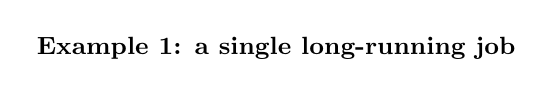
\begin{tikzpicture}[x=0.36mm, y=5.5mm]
  \node[anchor=west, font=\small\bfseries] at (-60,3.9) {Example 1: a single long-running job};
  \prows
  \ganttrow{3}{}{0/10/A}
  \ganttrow{2}{}{10/30/A}
  \ganttrow{1}{}{30/70/A}
  \ganttrow{0}{}{70/150/A, 150/230/A, 230/310/A}
  \ganttaxis{0}{0,30,70,150,230,310}
\end{tikzpicture}

\vspace{3mm}
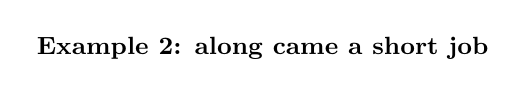
\begin{tikzpicture}[x=0.36mm, y=5.5mm]
  \node[anchor=west, font=\small\bfseries] at (-60,3.9) {Example 2: along came a short job};
  \prows
  \ganttrow{3}{}{0/10/A, 150/160/B}
  \ganttrow{2}{}{10/30/A, 160/180/B}
  \ganttrow{1}{}{30/70/A}
  \ganttrow{0}{}{70/150/A, 180/260/A, 260/310/A}
  \ganttaxis{0}{0,30,70,150,180,260,310}
\end{tikzpicture}

\vspace{3mm}
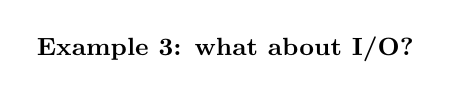
\begin{tikzpicture}[x=0.36mm, y=5.5mm]
  \node[anchor=west, font=\small\bfseries] at (-60,3.9) {Example 3: what about I/O?};
  \prows
  \ganttrow{3}{}{0/10/A, 150/151/B, 231/232/B}
  \ganttrow{2}{}{10/30/A}
  \ganttrow{1}{}{30/70/A}
  \ganttrow{0}{}{70/150/A, 151/231/A, 232/310/A}
  \ganttaxis{0}{0,30,70,150,231,310}
\end{tikzpicture}
\caption{MLFQ with time slices $10$, $20$, $40$, $80$ (after slides 156--158). Tick $10$ is omitted for space.}
\label{fig:mlfq}
\end{figure}

\begin{example}[MLFQ at Work]
  \label{ex:mlfq}
  \Cref{fig:mlfq} shows three scenarios.
  \begin{enumerate}
    \item \emph{A single long-running job.} A uses up its slice at every level and sinks to priority $0$, where it receives slices of $80$. Long-running jobs get a large time slice, which reduces context switching.
    \item \emph{Along came a short job.} B arrives at time $150$ and needs $30$. It enters at priority $3$, preempting A, and finishes within two levels at time $180$, after which A resumes. Short jobs run first---MLFQ approximates SJF without knowing job lengths in advance.
    \item \emph{What about I/O?} B is I/O-bound: it uses the CPU for $1$ unit at a time and then waits for I/O. Since it always gives up the CPU before its slice is up, it stays at priority $3$ and gets the CPU as soon as it wants it. I/O-bound jobs have a higher priority to access the CPU.
  \end{enumerate}
\end{example}

The scheme has two limitations. Long-running jobs may starve if there are too many interactive jobs. And a program may change its behavior over time: a job that computes for a long time when it starts and becomes interactive afterwards has already sunk to the bottom and is punished forever. Both are fixed by a \emph{priority boost}: after some time period, move all jobs to the highest priority.

\begin{keypoint}[The Rules of MLFQ]
  \begin{enumerate}
    \item If $\text{Priority}(A) > \text{Priority}(B)$, A runs (B does not).
    \item If $\text{Priority}(A) = \text{Priority}(B)$, A and B run round-robin using the time slice of their queue.
    \item When a job enters the system, it is placed at the highest priority (the topmost queue).
    \item Once a job uses up its time slice at a given level, its priority is reduced (it moves down one queue).
    \item After some time period, move all the jobs in the system to the topmost queue.
  \end{enumerate}
\end{keypoint}

MLFQ observes how jobs behave over time and prioritizes them accordingly. It delivers excellent overall performance, similar to SJF and PSJF, for short-running interactive jobs, and it is fair and makes progress for long-running CPU-intensive workloads. Many modern operating systems therefore use a form of MLFQ as their base scheduler.

\begin{keypoint}[Summary]
  There is no best or standard scheduling algorithm, partly because we cannot predict the CPU requirement of a process, we do not even know whether a job will eventually terminate, and online scheduling is NP-hard. Linux has used the \emph{Completely Fair Scheduler} (CFS), a dynamic priority algorithm based on red-black trees, since kernel 2.6.23.
\end{keypoint}

\subsection{(SUPPLEMENT) Further Topics}
\label{sec:sched-further}

\paragraph{Why SJF is optimal.} When all jobs arrive together and their lengths are known, nonpreemptive SJF minimizes the average wait time, and hence the average turnaround time. Exchange argument: if a longer job runs immediately before a shorter one, swapping the two shortens the short job's wait by more than it lengthens the long job's, strictly reducing the total. An optimal schedule therefore has no ``long before short'' adjacent pair. With staggered arrivals, PSJF---also called shortest remaining time first (SRTF)---is optimal for average turnaround time.

\paragraph{SJF needs to know the future.} Real systems do not know how long a job will run. The classic remedy predicts the next CPU burst by exponential averaging of past bursts, $\tau_{n+1} = \alpha t_n + (1 - \alpha)\tau_n$, where $t_n$ is the length of the $n$-th burst. MLFQ sidesteps prediction: it observes instead of guessing.

\paragraph{A typo on slide 139.} The numerator of the average turnaround time reads $100 + 110 + 120$; the turnaround times are $A = 100$, $B = 100$, $C = 110$, and $(100 + 100 + 110)/3 = 103.33$. The result on the slide is correct.

\paragraph{Why CPU utilization is a poor metric.} A busy CPU is not necessarily doing useful work: context switches, spinning, and page faults all keep it busy. Utilization near $100\%$ may also mean the system is overloaded and response times are degrading.

\paragraph{Gaming rule 4.} Under ``drop a level once the time slice is used up'', a program can issue a pointless I/O just before its slice expires and stay at the top level forever, monopolizing the CPU. OSTEP's fix is to account for the \emph{total} CPU time a job uses at a level: once it exhausts its allotment it moves down, however many times it gave up the CPU in between.

\paragraph{How CFS is ``completely fair''.} CFS has no fixed time slices. It tracks a \emph{virtual runtime} \code{vruntime} per process---actual runtime scaled by a weight derived from the nice value---and always runs the process with the smallest \code{vruntime}. Runnable processes are kept in a red-black tree keyed by \code{vruntime}; the leftmost node, cached, is the next to run, so picking is $O(1)$ and insertion $O(\log n)$. An I/O-bound process accumulates no \code{vruntime} while sleeping and is near the front when it wakes, much like MLFQ's preference for I/O-bound jobs. Since Linux 6.6, CFS has been replaced by the EEVDF (Earliest Eligible Virtual Deadline First) scheduler.

\paragraph{Priorities in Linux.} Ordinary processes are weighted by their \emph{nice value}, from $-20$ (highest) to $19$ (lowest): \code{nice -n 10 ./job}, \code{renice}. Real-time processes use separate policies, \code{SCHED\_FIFO} (FCFS within a priority, no time slice) and \code{SCHED\_RR} (round-robin within a priority), which always take precedence over ordinary processes; \code{chrt} sets them.

\paragraph{State letters in \code{ps}.} \code{R} is running or ready (Linux does not distinguish them; both are on the run queue), \code{S} interruptible sleep, \code{D} uninterruptible sleep, \code{T} stopped (e.g., by \code{SIGTSTP}), and \code{Z} zombie. A process in state \code{D} cannot be killed even with \code{SIGKILL}; the classic case is a process stuck on an unresponsive NFS mount.

\paragraph{Hidden costs of a context switch.} Switching address spaces invalidates the cached translations in the TLB (unless the hardware tags entries with PCID/ASID), and the new process starts with a cold cache. These costs often exceed saving and restoring registers. Switching between \emph{threads} of the same process needs no change of memory map and is therefore cheaper.

\paragraph{Priority inversion.} A low-priority process holds a lock that a high-priority process waits for, while a medium-priority process keeps preempting the low-priority one---so the high-priority process is starved indirectly by the medium one. This repeatedly reset the Mars Pathfinder in 1997. The fix is \emph{priority inheritance}: the lock holder temporarily inherits the priority of the highest-priority waiter.



\appendix
\chapter{System Call Reference}
\label{app:syscalls}

The process-management calls used in these notes, with the section where each is discussed.

\begin{center}
\small
\begin{tabular}{>{\ttfamily}l p{0.5\linewidth} l}
  \toprule
  \normalfont Call & What it does & See \\
  \midrule
  getpid(), getppid() & PID of the caller, PID of its parent & \Cref{sec:fork} \\
  fork() & clone the caller; returns the child's PID in the parent, $0$ in the child, $-1$ on failure; memory is shared copy-on-write & \Cref{sec:fork,sec:internals} \\
  execve(), exec*() & replace the program the process runs; does not return on success; keeps the PID and the fd table & \Cref{sec:fork,sec:internals} \\
  exit() & free memory, close files, leave a zombie, send \code{SIGCHLD} to the parent & \Cref{sec:internals} \\
  wait(), waitpid() & block until a child terminates and reap it; $-1$ if there are no children & \Cref{sec:fork,sec:internals} \\
  dup2(old, new) & make descriptor \code{new} refer to the open file of \code{old}; the basis of redirection & \Cref{sec:kernel} \\
  kill(pid, sig) & send a signal to a process; \code{raise(sig)} sends it to the caller & \Cref{sec:signals} \\
  signal(sig, h) & install a handler and return the old one; not possible for \code{SIGKILL} and \code{SIGSTOP} & \Cref{sec:signals} \\
  pause() & block until a handled or terminating signal arrives & \Cref{sec:signals} \\
  alarm(n), setitimer() & one-time or periodic timer delivering \code{SIGALRM} & \Cref{sec:signals} \\
  \bottomrule
\end{tabular}
\end{center}


\begin{thebibliography}{9}
\bibitem{CSAPP} R.~E. Bryant and D.~R. O'Hallaron. \emph{Computer Systems: A Programmer's Perspective}, 3rd edition. Pearson, 2015.
\bibitem{MOS} A.~S. Tanenbaum and H.~Bos. \emph{Modern Operating Systems}, 5th edition. Pearson, 2022.
\bibitem{OSC} A.~Silberschatz, P.~B. Galvin, and G.~Gagne. \emph{Operating System Concepts}, 10th edition. Wiley, 2018.
\bibitem{OSTEP} R.~H. Arpaci-Dusseau and A.~C. Arpaci-Dusseau. \emph{Operating Systems: Three Easy Pieces}. Arpaci-Dusseau Books, 2018.
\end{thebibliography}

\end{document}
